\documentclass[a4paper,12pt]{report}

% --------------------------------------------------
%  Packages
% --------------------------------------------------
\usepackage[utf8]{inputenc}  % Support for UTF-8 encoding
\usepackage[english]{babel}  % English language support
\usepackage{amsmath,amssymb} % Math packages
\usepackage{geometry}        % Page geometry
\usepackage{setspace}        % Line spacing
\usepackage{graphicx}        % Insert images
\usepackage{hyperref}        % Hyperlinks in the PDF
\usepackage{float}           % Improved float handling
\usepackage{listings}        % Code listings
\usepackage{xcolor}

% Define JSON language for listings
\lstdefinelanguage{json}{
    basicstyle=\ttfamily\small,
    numbers=left,
    numberstyle=\tiny\color{gray},
    stepnumber=1,
    numbersep=5pt,
    showstringspaces=false,
    breaklines=true,
    frame=single,
    backgroundcolor=\color{gray!10},
    literate=
     *{0}{{{\color{blue}0}}}{1}
      {1}{{{\color{blue}1}}}{1}
      {2}{{{\color{blue}2}}}{1}
      {3}{{{\color{blue}3}}}{1}
      {4}{{{\color{blue}4}}}{1}
      {5}{{{\color{blue}5}}}{1}
      {6}{{{\color{blue}6}}}{1}
      {7}{{{\color{blue}7}}}{1}
      {8}{{{\color{blue}8}}}{1}
      {9}{{{\color{blue}9}}}{1}
      {:}{{{\color{red}:}}}{1}
      {,}{{{\color{red},}}}{1}
      {"}{{{\color{orange}"}}}{1},
    keywordstyle=\color{blue},
    stringstyle=\color{orange},
    commentstyle=\color{gray},
    morecomment=[l][\color{magenta}]{//},
}

% Page margins
\geometry{
    left=3cm,
    right=2.5cm,
    top=2.5cm,
    bottom=2.5cm
}

\lstset{
  basicstyle=\ttfamily\small,
  frame=single,
  breaklines=true,
  backgroundcolor=\color{gray!10},
  captionpos=b,
  numbers=left,
  numberstyle=\tiny\color{gray},
  keywordstyle=\color{blue},
  commentstyle=\color{gray},
  stringstyle=\color{red},
  showstringspaces=false,
  columns=fullflexible,
  language=bash
}

\setstretch{1.3}  % Line spacing

% --------------------------------------------------
%  Begin Document
% --------------------------------------------------
\begin{document}

% --------------------------------------------------
%  Title Page
% --------------------------------------------------
\begin{titlepage}
    \begin{center}
        \vspace*{1.5cm}

        % AUEB Logo
        
\includegraphics[width=0.9\textwidth]{./aueb_logo.png}\\[1cm]

        {\Large \textbf{Athens University of Economics and Business}}\\[0.5cm]
        {\large Department of Management Science and Technology}\\[1.5cm]

        {\Huge \textbf{Undergraduate Thesis}}\\[1.2cm]
        {\Large \textbf{Behavioral Profiling of Popular Messaging Apps Using Kernel-Level Tracing}}\\[2cm]

        \textbf{Student:}\\
        Foivos - Timotheos Proestakis\\
        Student ID: 8210126\\[1.5cm]

        \textbf{Supervisors:}\\
        Prof. Diomidis Spinellis \\
        Dr. Nikolaos Alexopoulos\\[1.5cm]

        \vfill
        \textbf{Submission Date:}\\
        \today
        \vspace*{1cm}
    \end{center}
\end{titlepage}
\clearpage


% --------------------------------------------------
%  Abstract
% --------------------------------------------------
\begin{abstract}
This thesis examines kernel-level tracing techniques to create behavioral profiles of popular messaging applications.
\end{abstract}
\clearpage

% --------------------------------------------------
%  Acknowledgments
% --------------------------------------------------
\chapter*{Acknowledgments}
\addcontentsline{toc}{chapter}{Acknowledgments}

I would like to express my gratitude to my supervisors, Prof. Diomidis Spinellis
and Dr. Nikolaos Alexopoulos, for their invaluable guidance, insightful feedback,
and continuous support throughout the duration of this thesis. Their expertise and
encouragement were instrumental in the successful completion of this work.

I would also like to sincerely thank my exceptional fellow students, Vangelis Talos
and Giannis Karyotakis, for their contribution, collaboration, and for being true companions
in this academic journey.

A special thanks goes to my family, whose unwavering support, both emotional and practical,
made this endeavor not only possible but also deeply meaningful. Their presence and
encouragement were a constant source of strength.

\clearpage
% --------------------------------------------------
%  Table of Contents
% --------------------------------------------------

\tableofcontents
\clearpage

% --------------------------------------------------
%  Introduction
% --------------------------------------------------
\chapter{Introduction}

Smartphones have become an integral component of modern society, with the number
of global users surpassing 5 billion and continuing to grow rapidly
\cite{DataReportal2025}. Among the dominant mobile platforms, Android—an
open-source operating system developed by Google—holds a stable global market
share of approximately 75 \% \cite{StatCounter2025}. Its open-source nature,
flexibility, and widespread adoption have cultivated a vast ecosystem of
applications that enhance user productivity and social interaction across various
domains.

Among these applications, messaging platforms such as WhatsApp, Telegram,
Facebook Messenger, and Signal have gained significant popularity, playing a
central role in both personal and professional communication. However, the
ubiquitous use of smartphones for such purposes has led to the accumulation of
sensitive personal data on user devices, including photos, contact lists, location
history, and financial information, thereby raising serious privacy and security
concerns \cite{ArsTechnica2018}.

Incidents such as Facebook’s unauthorized collection of SMS texts and call logs
from Android devices \cite{ArsTechnica2018} underscore the vulnerabilities within
existing mobile ecosystems. In response, regulatory frameworks like the General
Data Protection Regulation (GDPR) and national laws such as the UK Data
Protection Act 2018 aim to enforce principles of transparency, data minimization,
and user consent in data processing \cite{GDPR2016,UKDPA2018}.

Despite these legislative efforts, Android’s current permission management system
remains insufficient. Users frequently misinterpret the scope and implications of
the permissions they grant, inadvertently exposing sensitive data to misuse
\cite{CHI2024Permissions}.

Furthermore, while end-to-end encryption (E2EE) provides strong guarantees for content
confidentiality, it is neither a necessary nor sufficient condition for overall application
security. The effectiveness of E2EE depends heavily on implementation correctness,
device-level protections, and metadata handling practices \cite{arxiv2020metadata,
wired2023signalhack}. Messaging apps may still leak sensitive information through
metadata such as message timing, connection patterns, or system-level behavior—even
when message content is encrypted. Notably, recent work has demonstrated how compromised
implementations or poorly configured server components can undermine the protections
offered by E2EE protocols \cite{wired2023signalhack}.

To address these challenges, it is essential to analyze application behavior—that
is, the actual operations performed by an app, both in the foreground and
background. Research has shown that discrepancies often exist between user
expectations and actual app behavior, with applications executing hidden or
unauthorized tasks \cite{NDSS2025Mismatch}. Many detection techniques rely on the
assumption that user-interface (UI) elements accurately represent application
functionality, an assumption that is not always valid \cite{NDSS2025Mismatch}.

Behavioral-analysis methods are typically divided into static and dynamic
approaches. Static analysis examines application code without execution,
identifying known malicious patterns; however, it is susceptible to evasion
through obfuscation and polymorphism \cite{MDPI2023Obfuscation}. In contrast,
dynamic analysis evaluates applications during runtime, monitoring behaviors such
as system calls, resource consumption, and network activity
\cite{SciDirect2023Syscall}. Among these, system-call analysis is particularly
valuable, offering fine-grained visibility into application interactions with
hardware and OS-level services \cite{SciDirect2023Syscall}.

Kernel-level tracing is a powerful form of dynamic analysis, capable of capturing
low-level system interactions with high precision \cite{BPFroid2021}. Android is
built on a modified
Linux kernel that orchestrates resource management and system processes via
system calls \cite{AOSP2024Ftrace}. Tools such as \texttt{ftrace} and
\texttt{kprobes} enable developers and researchers to trace kernel-level function
calls, execution flows, and resource usage \cite{AOSP2024Ftrace,Kprobes2024}.

\texttt{Ftrace} is a built-in tracing utility within the Linux kernel, optimized
for performance and capable of monitoring execution latency and function-call
sequences. \texttt{Kprobes}, on the other hand, allows for dynamic instrumentation
of running kernels, enabling targeted probing of specific code locations during
runtime \cite{Kprobes2024}.

Applying kernel-level tracing to messaging applications, however, introduces
unique technical challenges. These apps typically exhibit complex,
multi-threaded behavior, frequent background processing, and diverse interactions
with system resources. Accurately profiling such behavior requires collecting and
interpreting high-volume, high-resolution kernel data \cite{BPFroid2021}.

Despite the growing research interest in Android security and behavioral
analysis, existing work has primarily focused on general application profiling or
malware detection. Few studies have concentrated specifically on behavioral
profiling of messaging apps using kernel-level data \cite{SLR2025Messaging}.
Meanwhile, recent reports concerning the usage of secure messaging apps such as
Signal by government and military officials have emphasized the urgent need for
transparent, robust behavioral-analysis mechanisms \cite{Politico2025Signal}.

To address these gaps, this thesis proposes a structured methodology for
profiling the behavior of popular messaging applications on Android through
kernel-level tracing using \texttt{ftrace} and \texttt{kprobes}. The proposed
approach contributes a small but concrete step toward enhancing our understanding
of messaging app behavior on Android, with the broader aim of supporting future
efforts to strengthen user privacy and system transparency.

\section{Motivation and Problem Statement}

\paragraph{Motivation}
The motivation behind this research arises from the necessity to bridge existing
gaps between user expectations, regulatory compliance, and the actual operational
behavior of popular messaging applications. Messaging apps process extensive personal
data, creating substantial risks related to privacy violations and security breaches.
Recent incidents involving unauthorized data collection by prominent messaging
applications, along with revelations about governmental use of supposedly secure
messaging platforms, underscore significant concerns regarding transparency
and user trust.

\paragraph{Problem Statement}

Although prior work has explored various aspects of Android application behavior,
systematic analyses of messaging applications using kernel-level tracing remain
relatively scarce~\cite{DynamicSecurityAnalysis2023}. As a result, certain aspects
of runtime behavior—particularly those relevant to privacy and low-level system
interactions—are not yet well understood. This study seeks to modestly contribute
to this area by examining kernel-level traces of messaging apps under real-world
usage conditions, with the aim of informing future research and supporting more
transparent application behavior assessments.

\section{Research Objectives}

The specific research objectives addressed in this thesis are categorized as follows:

\subsection*{Primary Objectives}
\begin{itemize}
\item Identify potential violations of the principle of data minimization.
\item Analyze mismatches between granted permissions and real-time resource usage.
\item Detect unauthorized or hidden access to sensitive user data.
\item Compare the behavioral profiles of privacy-focused apps (e.g., Signal)
and more commercial alternatives.
\end{itemize}

\subsection*{Analytical and Technical Sub-Objectives}
\begin{itemize}
\item Record the actual kernel-level behavior of widely used messaging applications.
\item Develop a tracing and profiling framework using ftrace and kprobes.
\item Classify system calls into functional categories (file access, networking, IPC).
\item Monitor transitions between app states (idle, active, background).
\item Collect and analyze kernel-level usage statistics per application.
\item Implement a web-based dashboard for behavior visualization.
\end{itemize}

\subsection*{Broader Goals}
\begin{itemize}
\item Enhance transparency in how messaging apps behave at system level.
\item Improve user awareness of hidden behaviors executed in the background.
\item Demonstrate the value of kernel-level tracing for security and privacy evaluation.
\item Provide a structured and reproducible methodology for privacy-respecting
behavior analysis.
\end{itemize}

\section{Research Questions}
Based on the motivation and objectives, this thesis aims to address the following
research questions:

\vspace{0.5em}
\noindent\fbox{\parbox{\textwidth}{
\textbf{Q1.} What kernel-level operations do popular messaging applications perform
during normal usage?
}}

\vspace{0.5em}
\noindent\fbox{\parbox{\textwidth}{
\textbf{Q2.} Are there deviations between the declared permissions of these
applications and their actual behavior at runtime?
}}

\vspace{0.5em}
\noindent\fbox{\parbox{\textwidth}{
\textbf{Q3.} Can kernel-level tracing techniques identify unexpected or potentially
invasive operations performed without user interaction?
}}

\vspace{0.5em}
\noindent\fbox{\parbox{\textwidth}{
\textbf{Q4.} How does the behavior of privacy-focused apps compare to that of
commercial messaging platforms at the kernel level?
}}

\vspace{0.5em}
\noindent\fbox{\parbox{\textwidth}{
\textbf{Q5.} What kind of patterns in system calls can be used to characterize
privacy-relevant behavior?
}}


\section{Limitations}

To provide a realistic perspective on the scope of this thesis, we distinguish between
constraints that stem from practical project conditions and limitations that are
inherent to kernel-level behavioural research.

\subsection*{Project-Specific Constraints}

\begin{itemize}
    \item \textbf{Timeframe}: The study was conducted within the schedule of an
    undergraduate thesis, limiting the breadth of experiments (e.g., number of
    devices, data-collection days, and repetitions).
    \item \textbf{Hardware Diversity}: Tracing was performed on a small set of
    consumer devices; the results may not generalise to custom ROMs, tablets, or
    low-end hardware.
    \item \textbf{App Selection Bias}: Only three high-profile messaging apps
    (WhatsApp, Telegram, Signal) were analysed, excluding niche or region-specific platforms.
    \item \textbf{Resource Budget}: Storage, processing power, and time for
    post-processing large trace files were constrained by the available personal
    infrastructure.
\end{itemize}

\subsection*{Domain and Methodological Constraints}
\begin{itemize}
    \item \textbf{Semantic Gap}: Kernel traces expose low-level events (syscalls, Binder transactions) but lack direct mapping to high-level user actions, complicating interpretation.
    \item \textbf{Trace Volume}: High-frequency events can generate gigabyte-scale logs; aggressive filtering risks losing context, whereas full capture challenges storage and analysis pipelines.
    \item \textbf{Root Access Requirements}: The use of \texttt{kprobes} and access to \texttt{debugfs} requires root privileges, limiting applicability on production devices. While suitable for research, real-world deployment would require alternative mechanisms.
    \item \textbf{Noise in Dynamic Tracing}: Background services, OS updates, and vendor processes introduce variability that may mask or mimic app-specific behaviour.
\end{itemize}

\section{Contributions of this Thesis}

\section{Thesis Outline}
This thesis is organized into the following chapters:

\begin{itemize}
    \item \textbf{Chapter 1 – Introduction:} Establishes the broader context of smartphone use, with emphasis on messaging applications and their privacy implications. Discusses the limitations of permission-based models and end-to-end encryption in ensuring transparency. Motivates the use of kernel-level tracing as a complementary analysis method. Presents the thesis motivation, problem statement, research objectives, research questions, and outlines the scope and limitations. Provides an overview of the thesis structure.

    \item \textbf{Chapter 2 – Related Work:} Surveys prior literature on Android application analysis, categorized into static analysis, user-space dynamic instrumentation, kernel-level tracing, and empirical studies on messaging app privacy. Discusses complementary methodologies such as fuzzing, formal verification, differential privacy, side-channel analysis, and human-subject studies. Critically examines strengths and limitations of each line of work and identifies a clear research gap in systematic, runtime profiling of encrypted messaging apps using kernel-level methods.

    \item \textbf{Chapter 3 – Technical Background:} Introduces technical foundations required to understand the system-level behaviour of Android apps. Covers the Android/Linux architecture, process lifecycle, Binder IPC, SELinux enforcement, and system call interface. Explains the tracing infrastructure (ftrace, kprobes) and their relevance for behavioral profiling. Reviews the internal structure of messaging apps and discusses the “semantic gap” between kernel events and user-level activity.

    \item \textbf{Chapter 4 – Methodology and System Design:} Details the experimental methodology and system architecture. Describes the device setup, trace instrumentation approach using ftrace and kprobes, and session design. Presents the trace parsing pipeline, data pre-processing, feature derivation, and app-state inference. Explains how behaviors are correlated with declared permissions and how the collected data is structured and visualized through a web-based interface.

    \item \textbf{Chapter 5 – Results:} Summarizes empirical findings from real-world usage of WhatsApp, Telegram, and Signal. Presents observed kernel-level behaviors, event frequencies, system-call categories, and deviations between permission declarations and actual system-level activity. Provides side-by-side comparisons, statistical summaries, and visualizations of privacy-relevant patterns, such as background I/O, Binder bursts, and network usage under idle conditions.

    \item \textbf{Chapter 6 – Discussion:} Interprets the results in relation to the original research questions. Reflects on the practical implications of the findings, particularly concerning transparency, metadata exposure, and the role of kernel instrumentation in privacy audits. Discusses known limitations such as root access requirements, semantic ambiguity of low-level traces, data volume constraints, and potential improvements to the framework.

    \item \textbf{Chapter 7 – Conclusions:} Recaps the main contributions of the thesis and the insights gained from the study. Emphasizes the value of kernel-level tracing as a supplementary privacy analysis tool. Outlines open questions and proposes future directions, including integration with app-layer tracing, broader app coverage, automated behavior classification, and extending the approach to other app categories.

    \item \textbf{Appendix A – Additional Data Tables:} Provides supplementary tables, charts, and event frequency breakdowns that support the results chapter. Includes statistics per app and per session, outlier cases, and system-call distribution matrices.

    \item \textbf{Appendix B – Code:} Contains excerpts from scripts and tools used during data collection and analysis, including shell scripts for instrumentation, Python code for parsing and filtering traces, and the configuration files for kprobes and ftrace session management.
\end{itemize}

% --------------------------------------------------
%  Chapter 2 – Related Work
% --------------------------------------------------
\chapter{Related Work}\label{ch:related}

The purpose of this chapter is twofold: (i) to synthesise the state of the art on Android
application analysis with an emphasis on kernel–level tracing, and (ii) to
clearly demarcate the research gap that this thesis addresses.  The survey is
organised top‑down, gradually narrowing the focus from general program analysis
techniques to the specialised problem of privacy‑oriented behavioural
profiling of popular messaging applications.

\section{Static Analysis of Android Applications}
\label{sec:rw:static}

Static analysis inspects an \emph{APK}'s bytecode off-line, allowing security vetting to run quickly, deterministically, and at scale. It therefore plays a foundational role in Android app auditing, offering early detection of potential vulnerabilities without requiring runtime execution \cite{arzt2014flowdroid}.  Over the last decade, four interwoven research strands have successively expanded the scope and robustness of static techniques. These developments have progressively addressed the inherent limitations of static analysis—such as its inability to model inter-component interactions, and obfuscated code—by introducing more precise, scalable, and semantically enriched models. The key research directions can be grouped as follows:

\paragraph{(i) Privacy-oriented taint analysis.}
The first strand tracks information flows from sensitive \emph{sources} (e.g.\ GPS, contacts) to security-critical \emph{sinks} (e.g.\ network, logs).  \textbf{FlowDroid} introduced context-, flow-, field- and object-sensitivity together with an accurate lifecycle model, reducing false alarms dramatically.  On the \emph{DroidBench} suite it reaches 93\,\% recall and 86\,\% precision—outperforming both academic and commercial tools \cite{arzt2014flowdroid}—and it scales to large real-world apps such as Facebook, PayPal and LinkedIn.

\paragraph{(ii) Inter-component communication (ICC).}
Many leaks traverse process boundaries.  \textbf{IccTA} augments FlowDroid with an explicit ICC model, surpassing \textbf{Epicc} \cite{octeau2013epicc} and \textbf{CHEX} \cite{lu2012chex}—the latter targets component hijacking—on the \emph{ICC-Bench} suite.  \textbf{Amandroid} extends the idea further by building a full inter-component data-flow graph linking intents, callbacks and content providers; on 753 Play-store apps and 100 malware samples it uncovered previously unknown OAuth-token and intent-injection flaws while keeping analysis under one minute per APK \cite{wei2014amandroid}.

\paragraph{(iii) Obfuscation resilience.}
Reflection, dynamic loading and native libraries obscure control-flow and data types.  \textbf{DroidRA} resolves reflective calls through constant-propagation and rewrites them into direct invocations, boosting FlowDroid’s precision on reflection benchmarks by up to 60\,\% \cite{li2016droidra}.  \textbf{DexLEGO} reassembles bytecode collected at run time \cite{ning2019dexlego}, while \textbf{LibDroid} summarises taint propagation inside native libraries \cite{libdroid2022}; together they progressively widen the statically visible attack surface.

\paragraph{(iv) Learning-based malware detection.}
Moving beyond handcrafted rules, \textbf{Drebin} extracts lightweight syntactic features—permissions, intent actions, API calls—and detects malware with 94\,\% accuracy and 1\,\% false positives on 5\,560 samples \cite{arp2014drebin}.  Deep networks now dominate: \textbf{DL-AMDet} combines CNN-BiLSTM embeddings with an auto-encoder to reach 99.9\,\% accuracy on public datasets \cite{nasser2023dlamdet}.  Nonetheless, limited interpretability and training-set bias hinder deployment in high-assurance pipelines.

\medskip
\noindent\textbf{Synthesis.}
Static analysis has achieved substantial advances in precision and scale, yet it remains constrained by its inability to observe runtime-specific behavior, implicit flows, or obfuscated execution paths. These blind spots—especially critical in privacy contexts—have motivated a shift toward hybrid and dynamic approaches that can capture actual app behavior under real conditions.

\section{User-Space Dynamic Instrumentation}
\label{sec:rw:dynamic:user}

Whereas kernel tracing offers a \emph{system-wide} vantage, user-space dynamic
instrumentation injects probes \emph{inside} the app process, exposing rich
semantic context—class names, parameters, UI callbacks—without requiring a
custom kernel.  The literature has evolved along four complementary strands
that echo, in spirit, the structure reviewed for static analysis.

\paragraph{(i) System-call monitors.}
\textbf{DroidTrace} hooks every \texttt{ptrace} event to log the full
system-call stream and can \emph{force} rare branches to execute, increasing
coverage in malware analysis~\cite{zheng2014droidtrace}.  A later study
learns $n$-gram models that reconstruct high-level Android API invocations
purely from syscall sequences, demonstrating the semantic power of even
low-level traces~\cite{nisi2019syscall}.  These tools deploy on stock ROMs and
capture behaviour beneath any anti-hooking guard, yet they incur measurable
per-call overhead and cannot observe Java-level reflection or IPC content.

\paragraph{(ii) Dynamic binary instrumentation (DBI).}
Instruction-granular DBI engines such as \textbf{Pin} (ported to
ARM) enable fine-grained native tracing and custom analyses
(e.g.\ memory-safety checks) with mature tooling support, but
suffer from high runtime cost and outdated Android
support.  \textbf{QBDI} improves portability to modern ARM/Thumb-2
and withstands common packing techniques, although it remains native-only and
requires root privileges~\cite{qbdiblackhat2020}.

\paragraph{(iii) In-process hooking frameworks.}
\textbf{Frida} injects a tiny loader that JIT-compiles JavaScript hooks into
Java, JNI and native code, permitting live patching and interactive
experiments~\cite{frida2020}.  \textbf{DYNAMO} layers systematic diff-based
analysis on top of Frida to study framework evolution across Android
versions~\cite{dynamo2021}, while \textbf{InviSeal} hardens Frida against
detection, shrinking overhead to~$<\!3\%$ on UI benchmarks~\cite{inviseal2023}.
Yet all three struggle with tamper-aware apps and expose only the instrumented
process—cross-app flows, scheduler activity and kernel events remain hidden.

\paragraph{(iv) Sandbox and multi-layer profilers.}
Containerised sandboxes such as \textbf{C-Android} isolate each app inside a
Linux namespace and stream user-space logs for reproducible
testing~\cite{candroid2019}.  Emulation-centred pipelines (e.g.\ \textbf{DynaLog}
or DroidBox derivatives) automate large-scale malware triage by collecting
$\sim$100 runtime features in parallel VMs~\cite{dynalog2016}.  Although
high-throughput, these environments diverge from real-device timing,
miss in-kernel I/O, and are easily fingerprinted by sophisticated apps.

\medskip
\noindent\textbf{Synthesis.}
User-space instrumentation shines in \emph{semantic richness}, rapid
deployment and interactive control, making it ideal for annotating the coarse
kernel trace with method names, intent actions or UI context.  Its
weaknesses—visibility gaps below the syscall boundary, susceptibility to
anti-hooking defences and non-negligible overhead—underscore why kernel-level
tracing remains the authoritative foundation for our behavioural profiling of
messaging apps.  In our study, we therefore treat user-space hooks as an
\emph{auxiliary lens} to validate and enrich the low-level, system-wide evidence
captured by eBPF-based kernel monitors

\section{Kernel-Level Tracing on Android}
\label{sec:rw:kernel}

Kernel tracing hooks run beneath both the Java/ART runtime and the Linux
userland, recording system-wide events---syscalls, Binder transactions,
scheduler switches, network I/O---with negligible interference to the
application logic.  Such a viewpoint is pivotal for \emph{behavioural
profiling of end-to-end encrypted messaging apps}: once payloads are
ciphered in user space, only kernel footprints (e.g.\ TLS record bursts,
Binder-IPC patterns, power wakes) remain observable.  Like static analysis,
the literature has matured along four complementary strands.

\paragraph{(i) eBPF- and ftrace-based syscall/Binder collectors.}
\textbf{BPFroid} streams per-UID syscalls, Binder calls and network events
from \emph{stock} Android kernels to a real-time malware detector, achieving
$\sim$3\,\% overhead and 70\,\% Genome detection accuracy at run time
\cite{agman2021bpfroid}.  Earlier efforts, such as \textbf{ID-Syscall},
compiled a loadable kernel module to log syscall sequences for anomaly
detection on Android~4.x \cite{almuttawa2014syscall}.  These works show that
rich behavioural signals are available without modifying the firmware
image, yet they focus on binary classification rather than fine-grained
messaging-app semantics.

\paragraph{(ii) Network-centric and covert-channel tracing.}
Using vanilla \textit{ftrace}, Celik and Gligor detect
\emph{stegomalware} by spotting timing and packet-size irregularities in
kernel-level traces \cite{celik2021stego}.  Their methodology---correlating
scheduler, socket and power events---is transferable to instant-messaging
clients, but the study evaluates only artificial channels and omits Binder
traffic.

\paragraph{(iii) Hardware-assisted monitors.}
\textbf{HART} leverages ARM Embedded Trace Macro-cell (ETM) to stream
control-flow of binary-only kernel modules with zero software overhead
\cite{zhang2020hart}.  While ideal for diagnosing vendor drivers that gate
camera or GPU access in chat apps, ETM is often disabled on production
handsets and reveals no user-process context.

\paragraph{(iv) Production-scale, low-overhead tracing.}
Google’s \textbf{Perfetto} combines \emph{ftrace}, Binder and userspace
counters into multi-gigabyte traces that can be queried in SQL to dissect
app start-up and jank \cite{maganti2022perfetto}.  Complementarily,
\textbf{eMook} shows how per-PID filters inside eBPF eliminate tracing
overhead on unrelated processes, cutting system cost by 85\,\%
\cite{williams2024emook}.  These advances make week-long field studies of
battery-powered phones feasible but have yet to target security or
messaging use-cases explicitly.

\medskip
\noindent\textbf{Synthesis.}
Kernel-level instrumentation, although powerful, has five critical weaknesses:
\emph{(i) Semantic gap}—raw syscalls, Binder op-codes and network frames expose timing and sizes but no high-level intent;
\emph{(ii) Opaque content}—end-to-end encryption hides message bodies and most protocol metadata;
\emph{(iii) Privilege barrier}—enabling \texttt{kprobes}/eBPF typically requires \texttt{CAP\_SYS\_ADMIN}, a debug build, or root access;
\emph{(iv) Data volume}—high-frequency tracepoints (e.g.\ \texttt{sched\_switch}) can emit tens of MB\,s\(^{-1}\) unless filtered in-kernel; and
\emph{(v) Detectability}—sophisticated apps can query kernel debug files or eBPF counters to detect active probes and alter their behaviour.


\section{Privacy Studies on Messaging Applications}
\label{sec:rw:privacy-im}

End-to-end encryption neutralises classical content-centric attacks, but it
does not guarantee \emph{privacy}.  Over the last decade researchers have
investigated four complementary vectors through which popular messaging
apps still expose sensitive information.

\paragraph{(i) On-device artefacts and forensics.}
Early work focused on residual data stored locally.
Anglano’s systematic analysis of WhatsApp on Android~4.x recovered chat
databases, media thumbnails and contact lists even after user‐initiated
deletions \cite{anglano2015whatsapp}.
Subsequent studies extended the corpus to Telegram, Signal and Viber,
showing that cached profile photos, push-notification logs and SQLite WAL
files can reveal conversation partners and group identifiers
\cite{moltchanov2018telegram, obermeier2018signal}.
While modern versions encrypt local backups, notification side-channels
(e.g.\ Firebase tokens) remain an open avenue \cite{berezowski2020push}.

\paragraph{(ii) Network-level traffic analysis.}
A second strand exploits packet timing, size and sequence to infer user
actions without breaching encryption.
Pioneering work by Matic \emph{et al.} fingerprinted iMessage events
(send, read, typing) with $>90$ \% accuracy solely from TLS record
bursts \cite{matic2015iMessage}.
Apthorpe demonstrated similar leakage for Android IM apps over Wi-Fi
\cite{apthorpe2018smart}.
Recent machine-learning classifiers identify not only event types but also
multimedia uploads and voice-over-IP handshakes in QUIC traffic
\cite{lee2023quic}.
Countermeasures such as adaptive padding raise bandwidth by 8–14 \%
while mitigating most classifiers \cite{poblete2021defence}.

\paragraph{(iii) Contact-discovery and social-graph exposure.}
Many services hash user phone numbers and upload them for friend
discovery.  Tang \emph{et al.} reverse-engineered this protocol in
WhatsApp and estimated that an adversary can enumerate an EU-scale phone
space for \$500 of SMS fees \cite{tang2020whatsappHash}.
Kwon showed that Telegram’s “People Nearby” feature enables trilateration
of user location with meter-level accuracy \cite{kwon2021telegram}.  Signal
introduced private-set‐intersection with SGX enclaves to curb this vector,
yet follow-up work revealed side-channels via cache timing
\cite{marforio2022psi}.

\paragraph{(iv) Metadata policies and compliance audits.}
A complementary line audits whether apps meet their self-declared privacy
policies.  Egele’s longitudinal crawl of Telegram channels uncovered the
retention of deleted media on CDN edge nodes weeks after deletion
\cite{egele2019cdn}.
Bock dissected Signal’s sealed-sender protocol, confirming that only
sender and receiver persist in a 24-hour service log but flagging
exposure of push-token identifiers to Apple/Google \cite{bock2020sealed}.
Recent GDPR-oriented studies show that less than 40 \% of messaging apps
provide complete data-export facilities despite legal requirements
\cite{frolov2022gdpr}.


\medskip
\noindent\textbf{Synthesis.}
Existing studies either rely on intrusive forensics, controlled testbeds
or static policy analysis.  None combines \emph{kernel-level traces} with
the above insights to derive a live, system-wide privacy profile.
Our work closes this gap by correlating kprobe/ftrace events
(Binder calls, network bursts, wakelocks) with the metadata-leak patterns
catalogued in prior literature, delivering the first \emph{runtime}
taxonomy of privacy-relevant behaviours in WhatsApp, Telegram and Signal.


\section{Other Complementary Approaches}\label{sec:rw:other}

Beyond the four methodological pillars outlined earlier—static analysis, user-space dynamic instrumentation, kernel-level tracing, and empirical privacy audits—at least six additional research avenues have proven useful for dissecting the behaviour and privacy properties of mobile applications.

\paragraph{Grey-box fuzzing.}  Coverage-guided fuzzers such as \emph{AFL++} and cloud services like \emph{ClusterFuzz} generate mutated inputs that drive apps along rarely executed paths.  Although they do not rely on full program knowledge, they systematically surface crashes and logic errors that can later be inspected with dynamic or kernel monitors \cite{aflpp2023,clusterfuzz2020}.

\paragraph{Formal verification and model checking.}  Specification languages (e.g., TLA\textsuperscript{+}) combined with deductive verifiers (e.g., VeriFast) enable proofs of safety properties—such as correct handshake sequences in secure-messaging protocols or the absence of data races in JNI bridges—without collecting runtime traces \cite{antinyan2022noise,brack2019verifast}.

\paragraph{Privacy-preserving telemetry.}  Large-scale differential-privacy frameworks adopted by Apple and Google collect aggregate statistics while bounding individual leakage, offering population-level insight into security events without intruding on single devices \cite{erlingsson2019dpframework,apple2023ppac}.

\paragraph{Crowdsourced UI exploration.}  Robo-testing engines (e.g., Firebase Test Lab) drive accessibility events to map interface flows that static call graphs miss, producing semantic traces useful for regression testing and security auditing \cite{robo2018firebase}.

\paragraph{Physical side-channel analysis.}  Power-monitoring boards and electromagnetic probes can infer sensitive activity—such as encryption or radio bursts—without any software hooks, complementing software-based tracing when root or debugging privileges are unavailable \cite{emsec2023smartphone}.

\paragraph{Human-subject studies.}  Qualitative interviews and ethnographic methods shed light on adoption hurdles, configuration practices, and privacy norms that remain invisible to purely technical traces \cite{ngo2021signaladoption}.

Taken together, these complementary approaches can feed into kernel-centric measurement pipelines—for instance, by injecting fuzz-generated events into week-long traces or correlating power signatures with Binder activity—thereby enriching the behavioural picture without relying solely on any single layer of observation.

\section{Synthesis and Research Gap}\label{sec:rw:gap}

The preceding survey has examined four methodological pillars: \emph{(i)} static code analysis, \emph{(ii)} user-space dynamic instrumentation, \emph{(iii)} kernel-level tracing, and \emph{(iv)} empirical privacy studies on messaging applications.  Each strand contributes a distinct vantage on application behaviour, yet no single technique delivers a complete picture.  Below we distil their interplay and outline the remaining opportunities for improvement.

\subsection*{Synthesis of Current Methodologies}
\begin{itemize}
\item \textbf{Static analysis} offers breadth and determinism, uncovering dormant code paths and permission misalignments at scale.  Its reliability, however, is bounded by obfuscation, dynamic loading, and absent runtime context.
\item \textbf{User-space instrumentation} provides rich semantic detail—method names, parameters, UI state—and deploys quickly on stock devices.  This power is tempered by visibility gaps beneath the syscall layer, susceptibility to anti-hooking defences, and non-negligible overhead.
\item \textbf{Kernel-level tracing} records system-wide events with minimal perturbation, capturing activity that escapes sandboxed processes.  Yet it exposes only low-level artefacts (syscalls, Binder op-codes, I/O bursts) and therefore suffers from a semantic gap.
\item \textbf{Privacy audits of messaging apps} demonstrate that residual files, traffic metadata, and contact-discovery workflows leak sensitive information even under end-to-end encryption.  Most studies rely on targeted forensics or controlled testbeds rather than continuous observation on real devices.
\end{itemize}

Collectively, the literature indicates a gradual migration toward \emph{hybrid pipelines} that combine complementary techniques—e.g., leveraging static call-graphs to seed dynamic hooks, or enriching kernel traces with user-space context.  Despite this trend, a cohesive framework that correlates \emph{system-wide runtime evidence} with \emph{privacy-relevant semantics} remains under-explored, especially for widely-used, end-to-end-encrypted messaging services operating in the wild.

\subsection*{Identified Research Gap}
\begin{enumerate}
  \item \textbf{Runtime privacy profiling}. Existing kernel-level studies focus primarily on malware detection or performance debugging; they seldom translate low-level traces into privacy-oriented behavioural profiles.
  \item \textbf{Long-term, in-situ observation}. Prior work often relies on short laboratory sessions, emulators, or rooted devices. Evidence from week-long field measurements on stock handsets is scarce.
  \item \textbf{Correlating multi-layer signals}. Few frameworks align kernel events (e.g.\ Binder transactions, TLS bursts) with selective user-space context (e.g.\ intent actions, lifecycle callbacks).
  \item \textbf{Quantifying residual metadata leakage}. The literature documents individual side-channels but lacks a systematic taxonomy of leakage patterns observable solely from system-level traces.
\end{enumerate}

% --------------------------------------------------
%  Technical Background
% --------------------------------------------------

\chapter{Technical Background}

This chapter provides a detailed overview of technical background necessary for understanding the methodology and objectives of this thesis. First, it presents the architecture of the Android operating system, focusing particularly on the Linux-based kernel and how applications interact with it. Next, it discusses the behavior and privacy concerns related to messaging applications, highlighting known issues and relevant technical aspects. Furthermore, it outlines the advantages and limitations of static and dynamic analysis techniques and explores the role of system calls in behavior profiling. Finally, it reviews kernel-level tracing tools and techniques.
\section{Android Architecture and Kernel-Level Access}

\subsection{Android Software Stack Overview}
Android is a layered, open-source mobile operating system built on top of a customized version of the
Linux kernel. Its architecture is designed to be modular and extensible, supporting a wide range of
hardware while enforcing clear boundaries between components. The Android software stack consists
of four major layers: the Application Layer, the Java API Framework (commonly referred to as the
Application Framework), the Hardware Abstraction Layer (HAL), and the Linux Kernel.

The Application Layer hosts both system and user-installed applications.
These applications interact with the system via APIs exposed by the Android Framework.
The Java API Framework provides access to core system services such as activity management,
resource handling, content providers, and telephony. Services like \texttt{ActivityManager},
\texttt{WindowManager}, and \texttt{PackageManager} facilitate the lifecycle management and
orchestration of application behavior.

Beneath the framework lies the Android Runtime (ART), which executes application bytecode and optimizes it using ahead-of-time (AOT), just-in-time (JIT), or interpretation modes. Alongside ART are native libraries written in C/C++, including performance-critical components such as WebView, OpenSSL, and the Bionic libc. The Java Native Interface (JNI) allows managed Java/Kotlin code to call into these native libraries.

The HAL acts as a bridge between the Android Framework and the hardware drivers residing in the kernel. It defines standard interfaces that vendors implement to support various hardware components like audio, camera, sensors, and graphics. Since Android 10, Google introduced the Generic Kernel Image (GKI), which aims to further separate the vendor-specific hardware implementations from the core Linux kernel by introducing a stable kernel interface. This allows devices from different manufacturers to share a common kernel base while maintaining vendor-specific modules separately, simplifying updates and enhancing portability.

At the lowest level, the Linux kernel provides essential operating system services such as process scheduling, memory management, networking, and security enforcement. Android extends the kernel with additional features including the Binder IPC driver, ashmem (anonymous shared memory), and wakelocks to manage power usage. This kernel foundation ensures that resource access is isolated and controlled across all system layers.

\begin{figure}[H]
    \centering
    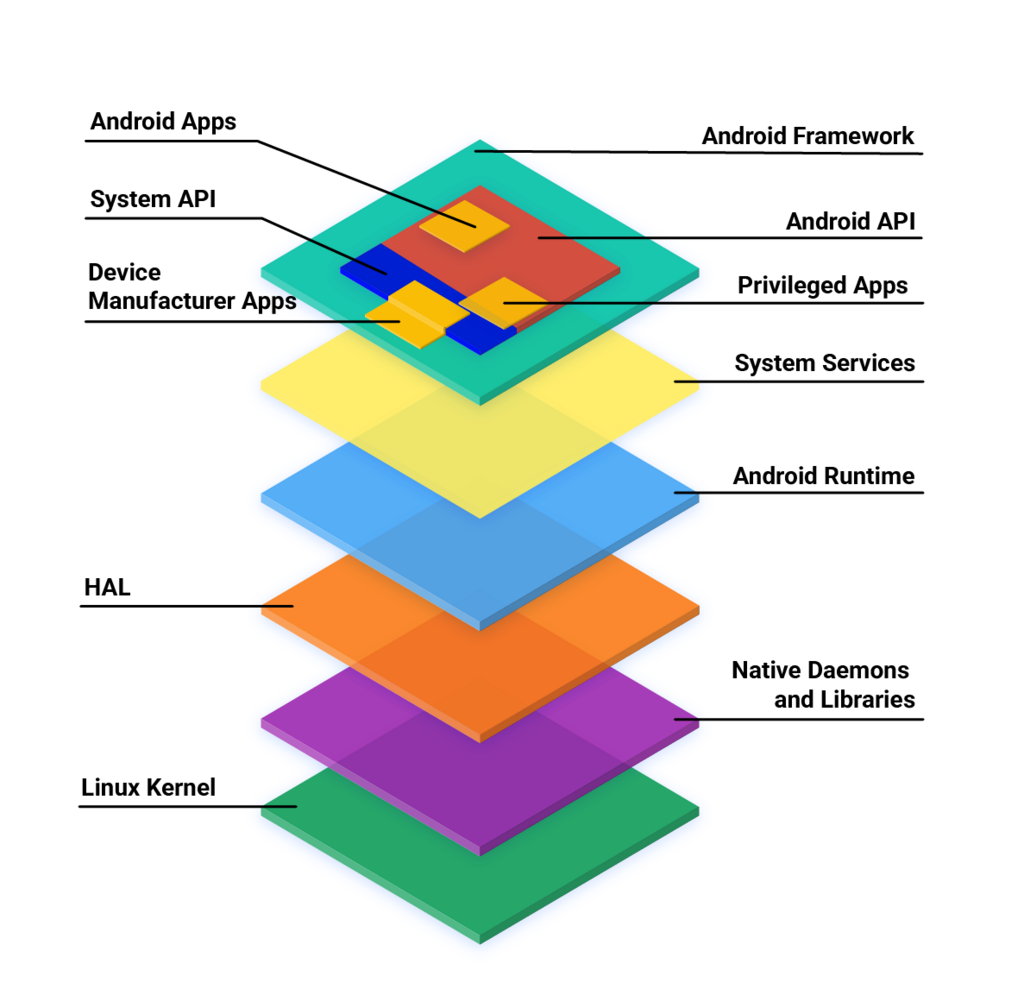
\includegraphics[width=0.75\textwidth]{android_stack_diagram.png}
    \caption{Updated Diagram of Android Software Stack (source: Android Developers Guide~\cite{androidplatformdoc}).}
    \label{fig:android_stack}
\end{figure}

\subsection{Application Layer and Process Lifecycle}
At the application layer, Android executes user and system applications packaged in APK format. Each APK includes compiled DEX bytecode, resources, native libraries, and a manifest file that defines app components and permissions. Apps run in sandboxed processes, each forked from the Zygote daemon—a minimal, preloaded system process that speeds up app launch time by sharing memory using copy-on-write.

The lifecycle of applications is centrally managed by the \texttt{ActivityManagerService} (AMS), which coordinates activity transitions, memory prioritization, and process states (foreground, background, cached). The \texttt{PackageManagerService} (PMS) handles component registration and permission declarations based on the manifest.

Apps follow a component-based model: Activities, Services, Broadcast Receivers, and Content Providers. These components interact with the system and one another via well-defined lifecycles and IPC through the Binder driver. Operations like binding to a service or launching an activity initiate system-level behavior—such as context switches or memory allocations—which are visible in syscall traces.

Binder IPC enables structured communication between app components and system services. Messages are serialized as Parcel objects, routed through the Binder driver, and trigger observable kernel events. These include context switches and transaction dispatches, which are measurable using tools like ftrace or kprobes.

Understanding transitions between app states (e.g., from idle to foreground) is vital in syscall-level profiling. For instance, foreground activation often leads to bursts of system calls such as \texttt{open()}, \texttt{stat()}, and \texttt{mmap()}—associated with UI initialization and resource loading. Such behaviors form recognizable patterns in kernel trace logs.

\subsection{Android Runtime, Native Layer, and JNI}
The Android Runtime (ART) executes application bytecode using a combination of ahead-of-time (AOT), just-in-time (JIT), and interpretation mechanisms. From a kernel-level tracing perspective, JIT-related memory operations may trigger system calls such as \texttt{mmap()}, \texttt{write()}, and \texttt{mprotect()}, as ART dynamically allocates memory for optimized code.

Beyond execution, ART interacts with the kernel to manage thread scheduling and memory access—behaviors that appear in system call traces. In dynamic analysis, such patterns can be correlated with app lifecycle events or anomalous execution spikes.

JNI further extends the runtime by enabling Java/Kotlin code to invoke native C/C++ libraries. These native operations often bypass standard framework controls, introducing low-level file, network, or cryptographic actions. This is particularly relevant for behavioral profiling, as native code may perform sensitive operations that differ from those visible at the Java level.

In the context of this thesis, which focuses on dynamic kernel-level analysis, capturing system interactions initiated by ART and JNI is essential. It enables the identification of execution phases or modules that deviate from expected behavior—especially in apps that rely heavily on native components for messaging, encryption, or background communication.
The sequence of events during JNI initialization is illustrated in Figure~\ref{fig:jni_init}.
It begins when the VM loads the application class, triggering a static initializer which invokes
the native \texttt{JNI\_OnLoad()} function. This function registers native methods and returns
the \texttt{JNI\_Version}, after which Android proceeds with the usual application lifecycle
(e.g., \texttt{onCreate()}) managed by the \texttt{ActivityManager}.
This interaction flow is especially relevant in behavioral analysis,
as native components may introduce low-level behavior patterns not observable through the Java layer alone.


\begin{figure}[H]
    \centering
    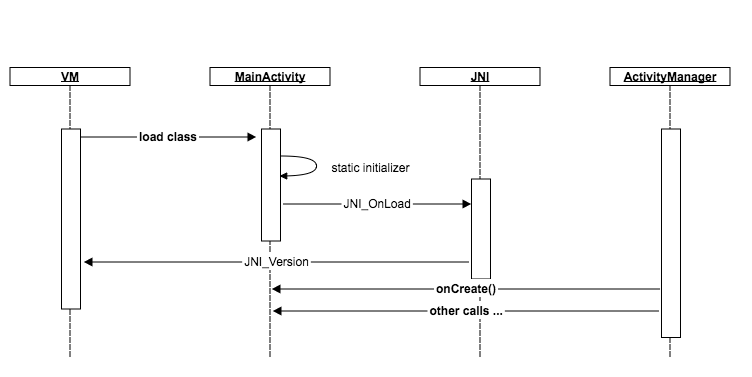
\includegraphics[width=0.85\textwidth]{jni_init_flow.png}
    \caption{Sequence diagram showing the JNI initialization flow in an Android application.}
    \label{fig:jni_init}
\end{figure}
\subsection{Linux Kernel Fundamentals in Android}
The Android operating system is built upon the Linux kernel, which serves as the foundational layer responsible for resource management, hardware abstraction, and secure process isolation. In the context of behavioral profiling and kernel-level tracing, the Linux kernel plays a pivotal role, as all application interactions with hardware and system resources are mediated through kernel functions and system calls.

A defining feature of the Linux kernel is its mediation of access to CPU, memory, file systems, and networking via the system call interface. When an Android application invokes a function that requires low-level operations (e.g., file access or sensor usage), it ultimately issues a system call that transitions the execution context from user space to kernel space. This transition boundary is where most behavioral artifacts manifest, making it ideal for tracing.

Android’s kernel incorporates additional components such as the Binder IPC driver, ashmem (for shared memory), and wakelocks (for power management). These Android-specific extensions generate kernel-level events observable by tracing tools. For example, Binder transactions facilitate inter-process communication and leave traceable patterns that can reveal background behavior of messaging apps.

Security is enforced through UID-based process separation, Linux namespaces, and SELinux Mandatory Access Control policies. Each app operates in its own sandbox and is assigned a unique UID, ensuring isolation at the kernel level. Deviations from expected isolation, especially in privileged system calls, may indicate abnormal or privacy-invading behavior.

Kernel tracing tools such as ftrace and kprobes allow developers to monitor kernel execution paths. Functions like \texttt{ksys\_open}, \texttt{\_\_sys\_sendmsg}, or \texttt{\_\_schedule} can be instrumented to capture low-level events such as file access, message transmission, or task switching. These traces are then analyzed to form behavioral profiles.

\textbf{Figure 4:} User Space to Kernel Space System Call Execution Path.

\subsection{System Calls and Kernel Interaction}
System calls are the primary interface through which Android applications interact with the kernel. Every high-level operation, such as reading a file or creating a socket, is translated into one or more system calls. These calls serve as an unfiltered log of what the application is actually doing, independent of its declared permissions or advertised functions.

In Android, system calls are usually invoked via the Bionic libc or directly through JNI bindings to native code. Behavioral profiling benefits from capturing these calls in real-time to identify patterns that indicate unexpected or excessive access to system resources.

Kernel tracing frameworks like ftrace and kprobes, and to a more advanced extent eBPF, can intercept and log system calls for offline or live analysis. For instance, an app issuing \texttt{sendto()} and \texttt{connect()} calls repeatedly in the background may be exfiltrating data without user knowledge.

\textbf{Figure 5:} Categorization of System Calls for Profiling: I/O, Network, IPC, Memory.

\subsection{ Android Security Model and Isolation Mechanisms}
Android enforces a layered security model combining Linux kernel features with user-space controls. Each application runs in its own sandbox, identified by a unique UID and GID, restricting file and device access. This is complemented by the use of SELinux in enforcing mode, which uses MAC policies to define allowable interactions between system components and applications.

Filesystem isolation further ensures that apps can only access their designated directories (e.g., \texttt{/data/data/{package\_name}}). Attempts to traverse or access other app spaces are blocked unless the app has elevated privileges or exploits kernel vulnerabilities.

System call filtering through seccomp restricts the range of calls an app can make, reducing the kernel's attack surface. From a profiling standpoint, observing unauthorized system calls or failed access attempts provides insight into potentially malicious or privacy-invasive behavior.

\textbf{Figure 6:} Android Security Layers: UID Isolation, SELinux, seccomp, Filesystem Sandboxing.

Relevant sources and additional references include official Android documentation, Linux kernel manuals, and peer-reviewed papers on Android system architecture and security.
\section{Messaging Apps: Characteristics  Privacy Implications}

\subsection{Functional and Architectural Overview}
Messaging applications are among the most widely used mobile software categories, providing real-time communication, media sharing, group messaging, and voice/video calling capabilities. Popular platforms such as Signal, Telegram, and Facebook Messenger serve billions of users globally, integrating deeply into daily communication routines.

Android, as the dominant mobile operating system, provides the primary distribution platform for these apps through the Google Play Store. According to public data \cite{statista2024messaging, googleplaydata2024}, Facebook Messenger has surpassed 5 billion downloads, Telegram exceeds 1.2 billion downloads, and Signal has more than 100 million installs. While usage varies by region, these numbers highlight the ubiquity and market penetration of messaging applications on Android devices.

Such widespread deployment across diverse hardware and Android configurations introduces heterogeneous behaviors in terms of network communication patterns, lifecycle management, and system-level operations. This diversity, combined with varying security practices among apps, renders them ideal candidates for behavioral profiling at the kernel level.

These applications typically rely on key Android components to support their functionality: foreground \texttt{Services} are used for persistent communication sessions, \texttt{Broadcast Receivers} handle asynchronous events such as network connectivity or message reception, and \texttt{Content Providers} facilitate access to structured data such as shared databases. All applications are packaged in APK format and structured using component declarations in the \texttt{AndroidManifest.xml} file.

Rather than detailing cryptographic implementations or privacy architectures here, which are explored in Section 2.2.3, this section focuses on the foundational aspects of app deployment, runtime behavior, and Android system integration that are relevant for low-level behavioral tracing.

\textbf{Figure 5:} Popular Messaging Apps by Feature Comparison and System Integration Characteristics.

\subsection{Privacy-Critical Behaviors and Resource Usage}
Messaging applications often initiate background services using components like \texttt{JobScheduler}, \texttt{AlarmManager}, and foreground services to maintain persistent communication channels—frequently waking the device from idle states using wakelocks \cite{androidwakelocks}.

Resource access is another key concern. Most messaging apps request access to sensitive resources such as contacts (\texttt{READ\_CONTACTS}), device location (\texttt{ACCESS\_FINE\_LOCATION}), microphone (\texttt{RECORD\_AUDIO}), and camera (\texttt{CAMERA}). While many of these are used legitimately during active user sessions (e.g., voice/video calls, media sharing), kernel-level traces often reveal such accesses occurring in the background without any visible UI activity—raising potential privacy concerns \cite{reardon2019leakage}.

Additionally, messaging apps rely on push notification services such as Firebase Cloud Messaging (FCM) or Google Cloud Messaging (GCM) to deliver messages. These services necessitate persistent TCP connections and background listeners that, when profiled, result in recurring system calls like \texttt{recvmsg()}, \texttt{poll()}, or \texttt{select()}. Furthermore, apps such as Facebook Messenger are known to incorporate third-party SDKs (e.g., for analytics or ads) that initiate background network connections and file I/O unrelated to core messaging functionality \cite{pi2018metadata}.

Metadata collection—such as timestamps, contact hashes, or device identifiers—is another privacy-relevant behavior. Even apps that implement strong encryption at the message content level (like Signal) may still generate system call activity that reflects metadata-related operations (e.g., \texttt{stat()}, \texttt{write()}, \texttt{getuid()}). In privacy-unfriendly apps, this is more pronounced and persistent \cite{signalprivacy2016}.

Finally, the use of native code through JNI can introduce kernel-visible activity that bypasses Android’s permission mediation layer. This is especially relevant for apps that offload cryptographic or media processing to native components. System call traces such as \texttt{mmap()}, \texttt{ioctl()}, and \texttt{openat()} often appear in these cases and can be captured using ftrace or kprobes.

These behaviors underscore the necessity of dynamic, syscall-level observation for detecting privacy-relevant activity and serve as foundational evidence in the behavioral profiling framework proposed in this thesis.

\textbf{Figure 6:} Typical System Call Patterns for Background Resource Access in Messaging Apps.

\subsection{Architectures, Privacy, and Cryptographic Models}
Messaging applications adopt distinct architectural and cryptographic frameworks that critically influence their privacy characteristics and observable behaviors at the kernel level. The majority of messaging platforms—including Signal, Telegram, and Facebook Messenger—use centralized client-server architectures, where backend servers handle communication routing, message storage, and authentication. Centralization supports multi-device synchronization and cloud storage but introduces privacy risks, such as metadata accumulation and continuous background socket activity (e.g., \texttt{connect()}, \texttt{poll()}, \texttt{recvmsg()}).

Signal utilizes a centralized yet privacy-focused architecture, relying exclusively on the Signal Protocol, a robust end-to-end encryption (E2EE) scheme ensuring forward secrecy, deniability, session-specific ephemeral keys, and the Double Ratchet algorithm for key management. The Double Ratchet combines a Diffie-Hellman key exchange and symmetric key cryptography, generating new encryption keys for every message sent, significantly enhancing security against key compromise \cite{signalwhitepaper}. Signal employs a custom Java implementation of the Signal Protocol known as libsignal, which provides cryptographic primitives and protocol management directly within Android applications, facilitating rigorous security auditing and simplifying integration. Kernel-level activities linked to Signal’s encryption involve system calls such as \texttt{getrandom()}, \texttt{mprotect()}, and \texttt{write()} during cryptographic operations. Signal's architecture avoids cloud synchronization and external dependencies, significantly reducing its syscall footprint.

Telegram implements a hybrid model, providing optional E2EE via "Secret Chats" but defaulting to server-side encryption. Standard conversations store plaintext messages centrally, enabling synchronization but increasing metadata exposure. This design results in elevated kernel activity, particularly frequent \texttt{send()}, \texttt{recv()}, and \texttt{stat()} calls for persistent synchronization and message retrieval.

Facebook Messenger exemplifies a privacy-limited centralized system, offering E2EE only within an opt-in "Secret Conversations" mode based on a derivative of the Signal Protocol. Default chats lack end-to-end encryption, incorporate numerous third-party SDKs for advertising and analytics, and generate extensive background system calls such as \texttt{open()}, \texttt{socket()}, \texttt{unlink()}, and \texttt{connect()}.

Storage models further distinguish these apps. Signal maintains exclusively local encrypted storage without cloud backups, minimizing kernel interactions. Telegram and Messenger utilize cloud synchronization for message histories, leading to increased kernel-level I/O operations (e.g., \texttt{open()}, \texttt{fsync()}, \texttt{stat()}).

Ephemeral messaging capabilities (disappearing messages) affect transient kernel behaviors, including short-lived file creation and memory operations like \texttt{madvise()}. Conversely, platforms that store logs or metadata generate repeated kernel interactions via persistent database accesses.

Finally, encryption key management significantly impacts syscall activity. Signal generates and securely stores keys locally using secure hardware or biometric-protected storage. Telegram and Messenger employ centralized key management, simplifying multi-device usage but requiring trust in backend infrastructure.

These architectural and cryptographic distinctions shape observable syscall behaviors, enabling kernel-level analysis to assess privacy implications effectively.

\textbf{Figure 7:} Comparative Analysis of Architectural and Cryptographic Models in Signal, Telegram, and Messenger.

\section{Static vs. Dynamic Analysis}

The security and behavioral analysis of Android applications typically leverages two main technical approaches: static and dynamic analysis. This section outlines the specific technical methodologies employed in each type of analysis, highlighting their mechanisms, strengths, and limitations from an implementation perspective.

\subsection{Static Analysis}

Static analysis involves the examination of application binaries and related artifacts without executing the code. Technically, this is performed through decompilation or disassembly of the Android APK files using tools such as JADX \cite{jadx}, Androguard \cite{androguard}, or MobSF \cite{mobsf}. These tools reverse engineer the application's bytecode to produce human-readable source code or intermediate representations, facilitating an inspection of declared permissions, class structures, method calls, and manifest configurations.

Static analysis typically includes extraction and inspection of AndroidManifest.xml to verify declared permissions and components, control-flow and data-flow analysis to detect potentially dangerous API usage and insecure coding patterns, and identification of embedded third-party libraries and hardcoded sensitive data such as keys or passwords.

However, static analysis is inherently limited by its inability to reflect runtime dynamics. It does not capture behaviors that depend on dynamic loading, obfuscation techniques, reflection, or native code invocation.

\subsection{Dynamic Analysis}

Dynamic analysis, conversely, involves observing and recording the application's runtime behavior within a controlled execution environment. This approach captures actual interactions with the Android operating system, including system calls, network activities, and file system operations. Dynamic analysis methods include both user-space instrumentation (using tools like Frida \cite{frida} and Xposed Framework \cite{xposed}) and kernel-level tracing.

Kernel-level dynamic analysis, specifically used in this thesis, employs system call tracing facilitated by Linux kernel tools such as \texttt{ftrace} \cite{ftrace}, \texttt{kprobes} \cite{kprobes}, and \texttt{debugfs} \cite{debugfs}. This technique involves enabling kernel-level probes to intercept and log specific system call invocations made by the application, capturing low-level operational details such as file accesses (\texttt{open()}, \texttt{read()}, \texttt{write()}), network communications (\texttt{connect()}, \texttt{sendto()}, \texttt{recvfrom()}), and process management activities, and recording the precise timing and sequence of system calls to reconstruct detailed behavioral profiles of application execution.

This low-level monitoring ensures comprehensive coverage of runtime behaviors, regardless of obfuscation or the execution of native code segments.

\subsection{Technical Comparison}

\begin{table}[h]
\centering
\begin{tabular}{|l|l|l|}
\hline
\textbf{Feature} & \textbf{Static Analysis} & \textbf{Dynamic Analysis (Kernel-level)} \\
\hline
Execution requirement & No execution & Runtime execution required \\ \hline
Tools examples & JADX, MobSF, Androguard & ftrace, kprobes, debugfs \\ \hline
Analyzed artifacts & APK, source code, manifest & System calls, runtime behaviors \\ \hline
Coverage of obfuscation & Limited or none & Comprehensive \\ \hline
Dynamic behaviors & Not captured & Fully captured \\ \hline
Detection of native code & Limited & Effective \\ \hline
Resource consumption & Typically lower & Higher (due to real-time monitoring) \\ \hline
Granularity & Moderate & High (syscall-level detail) \\ \hline
\end{tabular}
\caption{Technical Comparison of Static and Kernel-level Dynamic Analysis}
\label{table:comparison}
\end{table}

The inherent strengths of kernel-level dynamic analysis in capturing runtime behavior and its resilience to obfuscation techniques justify its selection as the primary methodological approach for this thesis.


\section{System Call Tracing and Behavioral Analysis}

Kernel-level system call tracing provides a low-level, ground-truth view of how Android applications interact with the operating system. In this section, we explore both the technical mechanisms available for capturing such interactions and the analytical methods used to extract meaningful behavioral insights—particularly in the context of privacy-sensitive mobile applications such as messaging platforms.

\subsection{Tracing Interfaces and Instrumentation Tools}
Several kernel-level tracing tools are available in Android and Linux-based systems, each offering a distinct trade-off between overhead, observability, and programmability:

\begin{itemize}
\item \textbf{ftrace}: Integrated into the Linux kernel, ftrace provides function-level and syscall-level tracing, context switches, scheduling events, and filtering by PID or syscall. It is accessible via \texttt{/sys/kernel/debug/tracing} and optimized for minimal overhead.
\item \textbf{kprobes and uprobes}: Support dynamic, on-the-fly instrumentation at both kernel and user-space function addresses. Useful for attaching probes at points like \texttt{do\_sys\_open}, logging file accesses and argument values.
\item \textbf{tracepoints}: Provide predefined hook points in the kernel source that offer safe, efficient monitoring of events such as process creation, file access, or scheduler activity. Often used with tools like perf or BCC.
\item \textbf{strace}: A user-space syscall tracer that uses ptrace to log syscall invocations. Ideal for debugging but with high overhead and poor stealth, making it unsuitable for continuous profiling.
\item \textbf{eBPF (Extended Berkeley Packet Filter)}: A modern programmable tracing interface allowing safe kernel extensions at runtime. It supports dynamic filtering, per-event logic, aggregation, and export to user space. Its adoption in Android is growing with newer kernels.
\end{itemize}

\textbf{Table 1: Comparison of Kernel Tracing Tools}


\subsection{Raw Trace Data and Post-Processing}
The output from syscall tracing tools typically consists of structured logs, such as:

\begin{verbatim}
<...>-1234 [000] .... 10000.123456: sys_enter_openat: dfd=AT_FDCWD filename="/data/user/0/app/cache/image.jpg"
\end{verbatim}

These logs capture syscall names, parameters, timestamps, and context (e.g., PID, thread state). To extract insights:

\begin{itemize}
\item Data is filtered and cleaned to isolate app-specific syscall events.
\item Features such as syscall frequency, argument patterns, and return codes are extracted.
\item Aggregated traces are converted to higher-level representations (e.g., n-grams, histograms) for machine learning or statistical analysis.
\end{itemize}

Post-processing typically involves parsing tools like Python scripts, custom Bash pipelines, or tools like \texttt{perf}, \texttt{bcc}, and \texttt{Sysdig}. These allow for correlation with app state (foreground/background), event type, and time windows.

\subsection{System Call Pattern Analysis and Behavioral Fingerprinting}

\subsubsection{Pattern Extraction Techniques}
To accurately analyze the behavior of Android messaging applications at the kernel level, it is crucial to extract meaningful patterns from the collected system call traces. After gathering raw trace data using kernel-level tracing mechanisms such as ftrace or kprobes \cite{gregg2019bpf}, the analysis pipeline proceeds with a structured set of extraction techniques.

Firstly, \textbf{trace preprocessing} is performed to filter irrelevant system calls that may be attributed to background system processes or kernel housekeeping tasks. This stage involves the normalization of syscall logs, removal of duplicates, and categorization into meaningful functional groups such as network operations (\texttt{sendto}, \texttt{recvmsg}), file operations (\texttt{open}, \texttt{read}, \texttt{write}), and memory operations (\texttt{mmap}, \texttt{mprotect}) \cite{tanenbaum2015modern}.

A fundamental step in pattern extraction is the use of \textbf{sliding window analysis} with N-grams, where sequences of consecutive system calls of fixed length (typically 3-5 syscalls) are extracted and analyzed for frequency. For instance, a recurring sequence like \texttt{open → mmap → sendto} can indicate frequent file accesses followed by network transmissions, a characteristic pattern for messaging activities such as sending multimedia files \cite{kim2019syscall}.

Moreover, we apply \textbf{temporal clustering} to detect bursts of system call activity, which are indicative of specific application behaviors like message sending, receiving notifications, or background synchronization. Clustering techniques such as DBSCAN or HDBSCAN help distinguish between typical and anomalous behavioral sequences based on temporal proximity \cite{ester1996density}.

Another valuable approach is constructing \textbf{system call frequency vectors}. Each trace is represented as a numerical vector, with dimensions corresponding to different system calls, facilitating quantitative comparisons between different sessions or different applications. This approach supports both exploratory analysis and automated classification tasks \cite{bishop2007pattern}.

Finally, to model the complex dependencies between system calls, \textbf{graph-based extraction methods} such as directed state-transition graphs are utilized. In these graphs, nodes represent individual syscalls, and directed edges capture the observed transitions between them. Analysis of such graphs, for instance via centrality measures, provides insights into dominant behavioral flows and significant transition points within an application's runtime \cite{newman2010networks}.

\subsubsection{Behavioral Fingerprinting}
Behavioral fingerprinting refers to constructing distinct behavioral signatures of applications based on their system call patterns. Given the kernel-level granularity of our data, these fingerprints provide robust indicators of application identity, operational phases, and potential privacy-related activities.

A \textbf{behavioral fingerprint} is formally defined as the set of characteristic system call sequences or frequency distributions uniquely associated with an application's operation. To create these fingerprints, multiple execution traces of the same application under controlled conditions (e.g., message sending, multimedia sharing, background synchronization) are aggregated. Frequent and consistent system call patterns are identified using techniques such as frequent subsequence mining or clustering \cite{han2022datamining}.

These fingerprints facilitate several critical analyses. For example, by comparing fingerprints across messaging applications such as Signal, Telegram, and Facebook Messenger, distinct operational behaviors emerge, highlighting differences in their privacy handling and background operations. Fingerprints based on syscall sequences like \texttt{stat → open → sendto} can reliably indicate data transmissions or potential data exfiltration events \cite{enck2014taintdroid}.

Further, fingerprints serve as powerful tools for anomaly detection. By establishing baseline fingerprints under normal operating conditions, deviations can be quickly identified, suggesting unusual behaviors such as increased network activity or unauthorized access to sensitive files. This method enables proactive identification of potential privacy infringements or malicious behavior, complementing traditional security mechanisms \cite{chandola2009anomaly}.

Practically, we represent fingerprints as frequency vectors, n-gram sequences, or transition graphs, each capturing distinct aspects of the application's behavior. Frequency vectors offer a straightforward numerical approach for quick comparisons, while n-gram sequences and transition graphs provide more detailed behavioral context.

Ultimately, behavioral fingerprinting based on kernel-level system call patterns enhances our understanding of application behavior, supports precise application identification, and significantly improves privacy and security analysis within the Android ecosystem \cite{felt2011androidprivacy}.



\subsection{Formal Security and Privacy Models}

The methodology and design decisions presented in this thesis are guided by formal theoretical frameworks for security and privacy. Specifically, we draw upon foundational concepts from Information Flow Control (IFC) and the Bell-LaPadula (BLP) security model, establishing a clear theoretical underpinning for monitoring and analyzing resource access at the kernel level.

\subsubsection{Information Flow Control (IFC)}

Information Flow Control (IFC) is a security paradigm aimed at managing how sensitive information propagates through a computing system. IFC systems enforce explicit policies to restrict data from flowing from sensitive sources (e.g., contacts database, microphone input) to less secure or unauthorized destinations (e.g., network interfaces, file storage). The goal is to prevent unintended or unauthorized information disclosure \cite{myers1999jflow,sabelfeld2003language}.

In the context of this thesis, sensitive databases such as \texttt{contacts2.db} or devices such as microphones and cameras serve as information sources with high confidentiality. Network sockets or files accessible to third-party apps can act as sinks. Our kernel-level tracing infrastructure implicitly implements an IFC-like monitoring mechanism, providing evidence of potential violations when unexpected information flows are observed.

\subsubsection{Bell-LaPadula Security Model (BLP)}

The Bell-LaPadula model is a foundational model in computer security developed to maintain data confidentiality by enforcing mandatory access control (MAC). The core of BLP consists of two primary rules:

\begin{itemize}
    \item \textbf{No Read Up (NRU)}: A subject cannot read data at a higher security level than its own.
    \item \textbf{No Write Down (NWD)}: A subject cannot write data to a lower security level, thus preventing leaks of confidential information.
\end{itemize}

Although BLP was originally developed for military-grade systems, its core principles are applicable to modern mobile platforms. In Android, for instance, apps operate with different privilege levels defined by sandboxing and permission models. A violation of BLP might occur if a low-privilege app manages to read camera or contacts data (a "read up"), or if it writes that data to shared, world-readable files (a "write down").

The tracing framework developed in this thesis enables the identification of such violations by observing which applications interact with which resources, and under what circumstances. While Android does not implement BLP directly, our system draws on its principles to guide the labeling and evaluation of access events.

\bigskip

By integrating insights from IFC and BLP, we are able to frame kernel-level observations within a broader security context, supporting the detection of anomalous and potentially dangerous behaviors through a policy-driven lens.



% --------------------------------------------------
%  Research Methodology
% --------------------------------------------------
\chapter{Methodology and System Design}

This thesis is part of a broader research effort investigating the security and behavioral analysis of Android applications at the kernel level. While the present work focuses on behavioral profiling for privacy analysis, other components of the research include detection mechanisms using machine learning, portability of tracing techniques across devices, and offset-agnostic instrumentation. These aspects are discussed in parallel efforts by the research team, but are outside the scope of this thesis.

Importantly, this thesis constitutes a natural extension of the SYSDROID framework, an earlier kernel tracing platform developed by Nikos Alexopoulos as part of a research initiative at the Athens University of Economics and Business. SYSDROID laid the foundation for dynamic system-level monitoring of Android applications using tools such as ftrace and kprobes, focusing on syscall-level logging and low-level behavioral capture. The architectural overview that follows is largely based on the design principles and modular structure introduced in that initial work, with substantial refinements, generalizations, and extensions introduced in the context of this thesis.

\section{Research Design}

The research design employs a kernel-level tracing approach to profile behavioral patterns of popular Android messaging applications without requiring app instrumentation. The primary goal is to transparently capture system-level activities, such as system calls, IPC, and network interactions, to detect privacy-sensitive behaviors. Kernel-level tracing was chosen over user-level or API-based approaches due to its transparency, accuracy, and non-invasive nature. Experiments were performed on a rooted Android device using Magisk and bootloader unlocking for kernel tracing filesystem (\texttt{tracefs}) access.

The study follows a minimal intervention, ``black-box'' methodology with no modifications to apps or OS components, focusing solely on kernel observations. Technical tools used include \texttt{ftrace}, \texttt{kprobes}, ADB, custom shell scripts, and Python scripts for parsing and processing trace data into structured formats (JSON).

An additional design decision was the use of \texttt{kprobes} and \texttt{ftrace} instead of more advanced or emerging technologies such as eBPF. This choice was primarily driven by the principle of simplicity, in line with Occam's razor---opting for the simplest effective solution when more complex alternatives are unnecessary. Since the research objectives could be fully met using established, low-level tracing tools, there was no compelling need to adopt or upgrade to more sophisticated frameworks. This approach facilitated ease of deployment, lower learning curve, and minimized potential system instability or compatibility issues, while still ensuring comprehensive data collection for the study's requirements.

Design principles such as reproducibility, low overhead, and the detection capability for IPC, sensitive resource access, and network activities are prioritized. A sliding window approach is applied for detailed temporal analysis.

Data quality is ensured via validation and heuristic cleaning to filter irrelevant daemon activities. Comprehensive downstream analysis, including statistical evaluation, visualization, and a web-based interface, will be thoroughly detailed in subsequent sections.

In particular, the tracing process is initiated through a set of \texttt{bash} scripts executed directly on the Android device. These scripts dynamically configure and activate \texttt{kprobes} and \texttt{tracepoints} to monitor relevant kernel-level events, targeting specific system calls and function entries of interest. The resulting raw trace data is collected from the \texttt{tracefs} interface and securely exported to the host system.

Once exported, custom Python scripts are used to process and clean the raw logs. These scripts apply PID-based filtering and heuristic techniques to isolate information flows originating from the specific messaging application under analysis, while removing noise introduced by unrelated background system processes. The cleaned data is transformed into structured formats such as JSON or CSV to support downstream processing.

The final stage of the pipeline involves visualization. Static visualizations are generated using Python plotting libraries (e.g., \texttt{matplotlib}), providing summary statistics and event distributions. In parallel, an interactive web-based visualization tool has been developed using \texttt{Flask} and \texttt{D3.js}. This interface offers dynamic filtering by PID, event type, and timestamps, along with timeline-based views and graph-based summaries of system interactions.
\section{Experimental Setup}

The experimental setup involves detailed technical preparation and precise procedures to ensure kernel-level tracing capability. The device selected was a OnePlus Nord CE 4 Lite (CPH2621, EU variant) running Android 15 (SDK 35). It supports System-as-Root (\texttt{isSAR=true}), features A/B partitioning (\texttt{isAB=true}), and includes an accessible ramdisk.

\subsection{Root Access and Boot Image Preparation}

The device was prepared for root access using Magisk, following guidelines from xda-developers. Developer Options, OEM Unlocking, and USB Debugging were activated. Android SDK Platform Tools were installed on the computer, with the path added to environment variables, enabling communication via ADB.

After obtaining the full OTA zip for the CPH2621 EU variant via Oxygen Updater, it was transferred to the computer and unpacked to extract the \texttt{payload.bin} file. Using Payload Dumper, the \texttt{boot image} was retrieved. The Magisk APK was then used to patch the image, and the resulting file was flashed to the appropriate partition.

The sequence of commands used during the rooting process is provided in Listing~\ref{lst:rooting-commands}.

\begin{lstlisting}[caption={Command Sequence for Rooting Procedure},label={lst:rooting-commands},numbers=left]
adb devices
adb reboot bootloader
fastboot flashing unlock
adb pull /sdcard/Download/OTA.zip
python payload_dumper.py payload.bin
fastboot flash boot_a magisk_patched-28100_4owcs.img
\end{lstlisting}

\subsection{ADB Setup and Execution Environment}

The ADB setup enabled detailed interaction between the computer and the rooted device, allowing the execution of custom shell scripts for tracing and Python scripts for detailed data parsing and cleaning. Issues regarding portability and trace events were tracked and resolved using a structured GitHub project setup.

This configuration ensured reliable kernel-level data collection, maintaining reproducibility, accuracy, and minimal system intrusion.

\subsection{Identifying Sensitive Database Files}

In order to monitor access to sensitive databases (such as \texttt{contacts2.db} or \texttt{mmssms.db}), each target file needed to be uniquely identified using its inode and device ID. The \texttt{stat} command was used to extract this metadata, which provided both the inode number and the major/minor device number of the filesystem hosting the file. An example command is shown in Listing~\ref{lst:db-stat}.

\begin{lstlisting}[language=sh,caption={Retrieving inode and device ID for a database file},label={lst:db-stat},numbers=left]
adb shell stat /data/data/com.android.providers.contacts/databases/contacts2.db
\end{lstlisting}

The output of this command includes the \texttt{Device}, \texttt{Inode}, and full path, which were stored as part of a JSON metadata mapping. These values were then used to match trace events against specific sensitive files during analysis.

\subsection{Device Node Mapping for Hardware Resources}

To associate trace events with hardware resources such as the camera, microphone, or NFC module, we identified the corresponding character device nodes exposed by the kernel. Each device node in \texttt{/dev} is linked to a major and minor number pair, which can be extracted from the \texttt{/sys/class/**/dev} entries. A loop was used to recursively enumerate device nodes and extract their metadata, as illustrated in Listing~\ref{lst:device-node-scan}.

\begin{lstlisting}[caption={Enumerating character and block devices with major:minor IDs},label={lst:device-node-scan},numbers=left]
adb shell
for f in $(find /sys/class/ -name dev); do
    echo "$f -> $(cat $f)"
done
\end{lstlisting}

Each output entry was parsed to associate paths like \texttt{/dev/video0}, \texttt{/dev/snd/pcmC0D0c}, or \texttt{/dev/nq-nci} with their respective major:minor IDs. These values were encoded using the formula shown in Listing~\ref{lst:devt-calc}.

\begin{lstlisting}[caption={Encoding device number using major and minor},label={lst:devt-calc},numbers=none]
dev_t = (major << 20) | minor
\end{lstlisting}

This encoding was used in the trace parser to associate low-level device accesses with high-level categories such as camera or audio input.

\subsection{Automation and Metadata Serialization}

To automate both processes, a collaborator (Giannis Karyotakis) contributed Bash and Python scripts that programmatically retrieved and serialized this metadata into structured JSON files. These mappings were then used during the trace parsing phase to enrich low-level kernel events with high-level semantic labels.

This structured and collaborative approach enabled high-fidelity kernel tracing while minimizing manual overhead and potential for error.
An excerpt of the structured metadata format is shown in Listing~\ref{lst:json-metadata}, demonstrating how each sensitive resource is uniquely identified by a combination of its inode, major/minor device numbers, and a descriptive label.

\begin{lstlisting}[caption={Serialized JSON metadata for sensitive resource mapping},label={lst:json-metadata},numbers=left]
{
  "contacts": {
    "st_dev16": 65102,
    "st_dev32": 266338382,
    "major": 254,
    "minor": 78,
    "inode": 9253,
    "path": "/data/data/com.android.providers.contacts/databases/contacts2.db",
    "description": "Contacts database"
  }
}
\end{lstlisting}

\section{System Architecture and Data Flow}

The system is architected as a multi-layered pipeline for capturing, processing, and analysing kernel-level behavioural data on Android devices. Figure~\ref{fig:architecture} illustrates the overall architecture and the principal data flow across its components.

At a high level, the pipeline begins with a mobile-side tracing engine, which leverages configurable instrumentation via \texttt{kprobes}, \texttt{tracefs}, and declarative tracing policies. The engine is supported by a resource resolution layer that augments raw trace events with context such as inode paths, socket identifiers, and mapping metadata. This layer plays a critical role in enabling high-level semantic interpretation of low-level events. In particular, it facilitates the identification of accesses to sensitive device resources such as the camera or microphone, as well as interactions with privacy-critical application components, including contact lists, messaging services, and storage providers.

The collected data is stored temporarily on the device and later transferred to the host system for processing. There, a sequence of Python utilities and analysis notebooks is employed to parse, filter, flatten, and segment the traces. These components enable information flow tracking for specific applications and generate both static and interactive outputs.

Visualisation is handled through a modular dashboard consisting of a Flask-based backend and a D3.js-driven frontend. This dashboard supports dynamic filtering, event inspection, and behavioural summaries via timeline and statistical charts.

Each component of the system—ranging from mobile-side tracing and contextual enrichment, to host-side processing and web-based presentation—will be described in detail in the following sections, with direct reference to the layers depicted in Figure~\ref{fig:architecture}.
\begin{figure}[H]
\centering
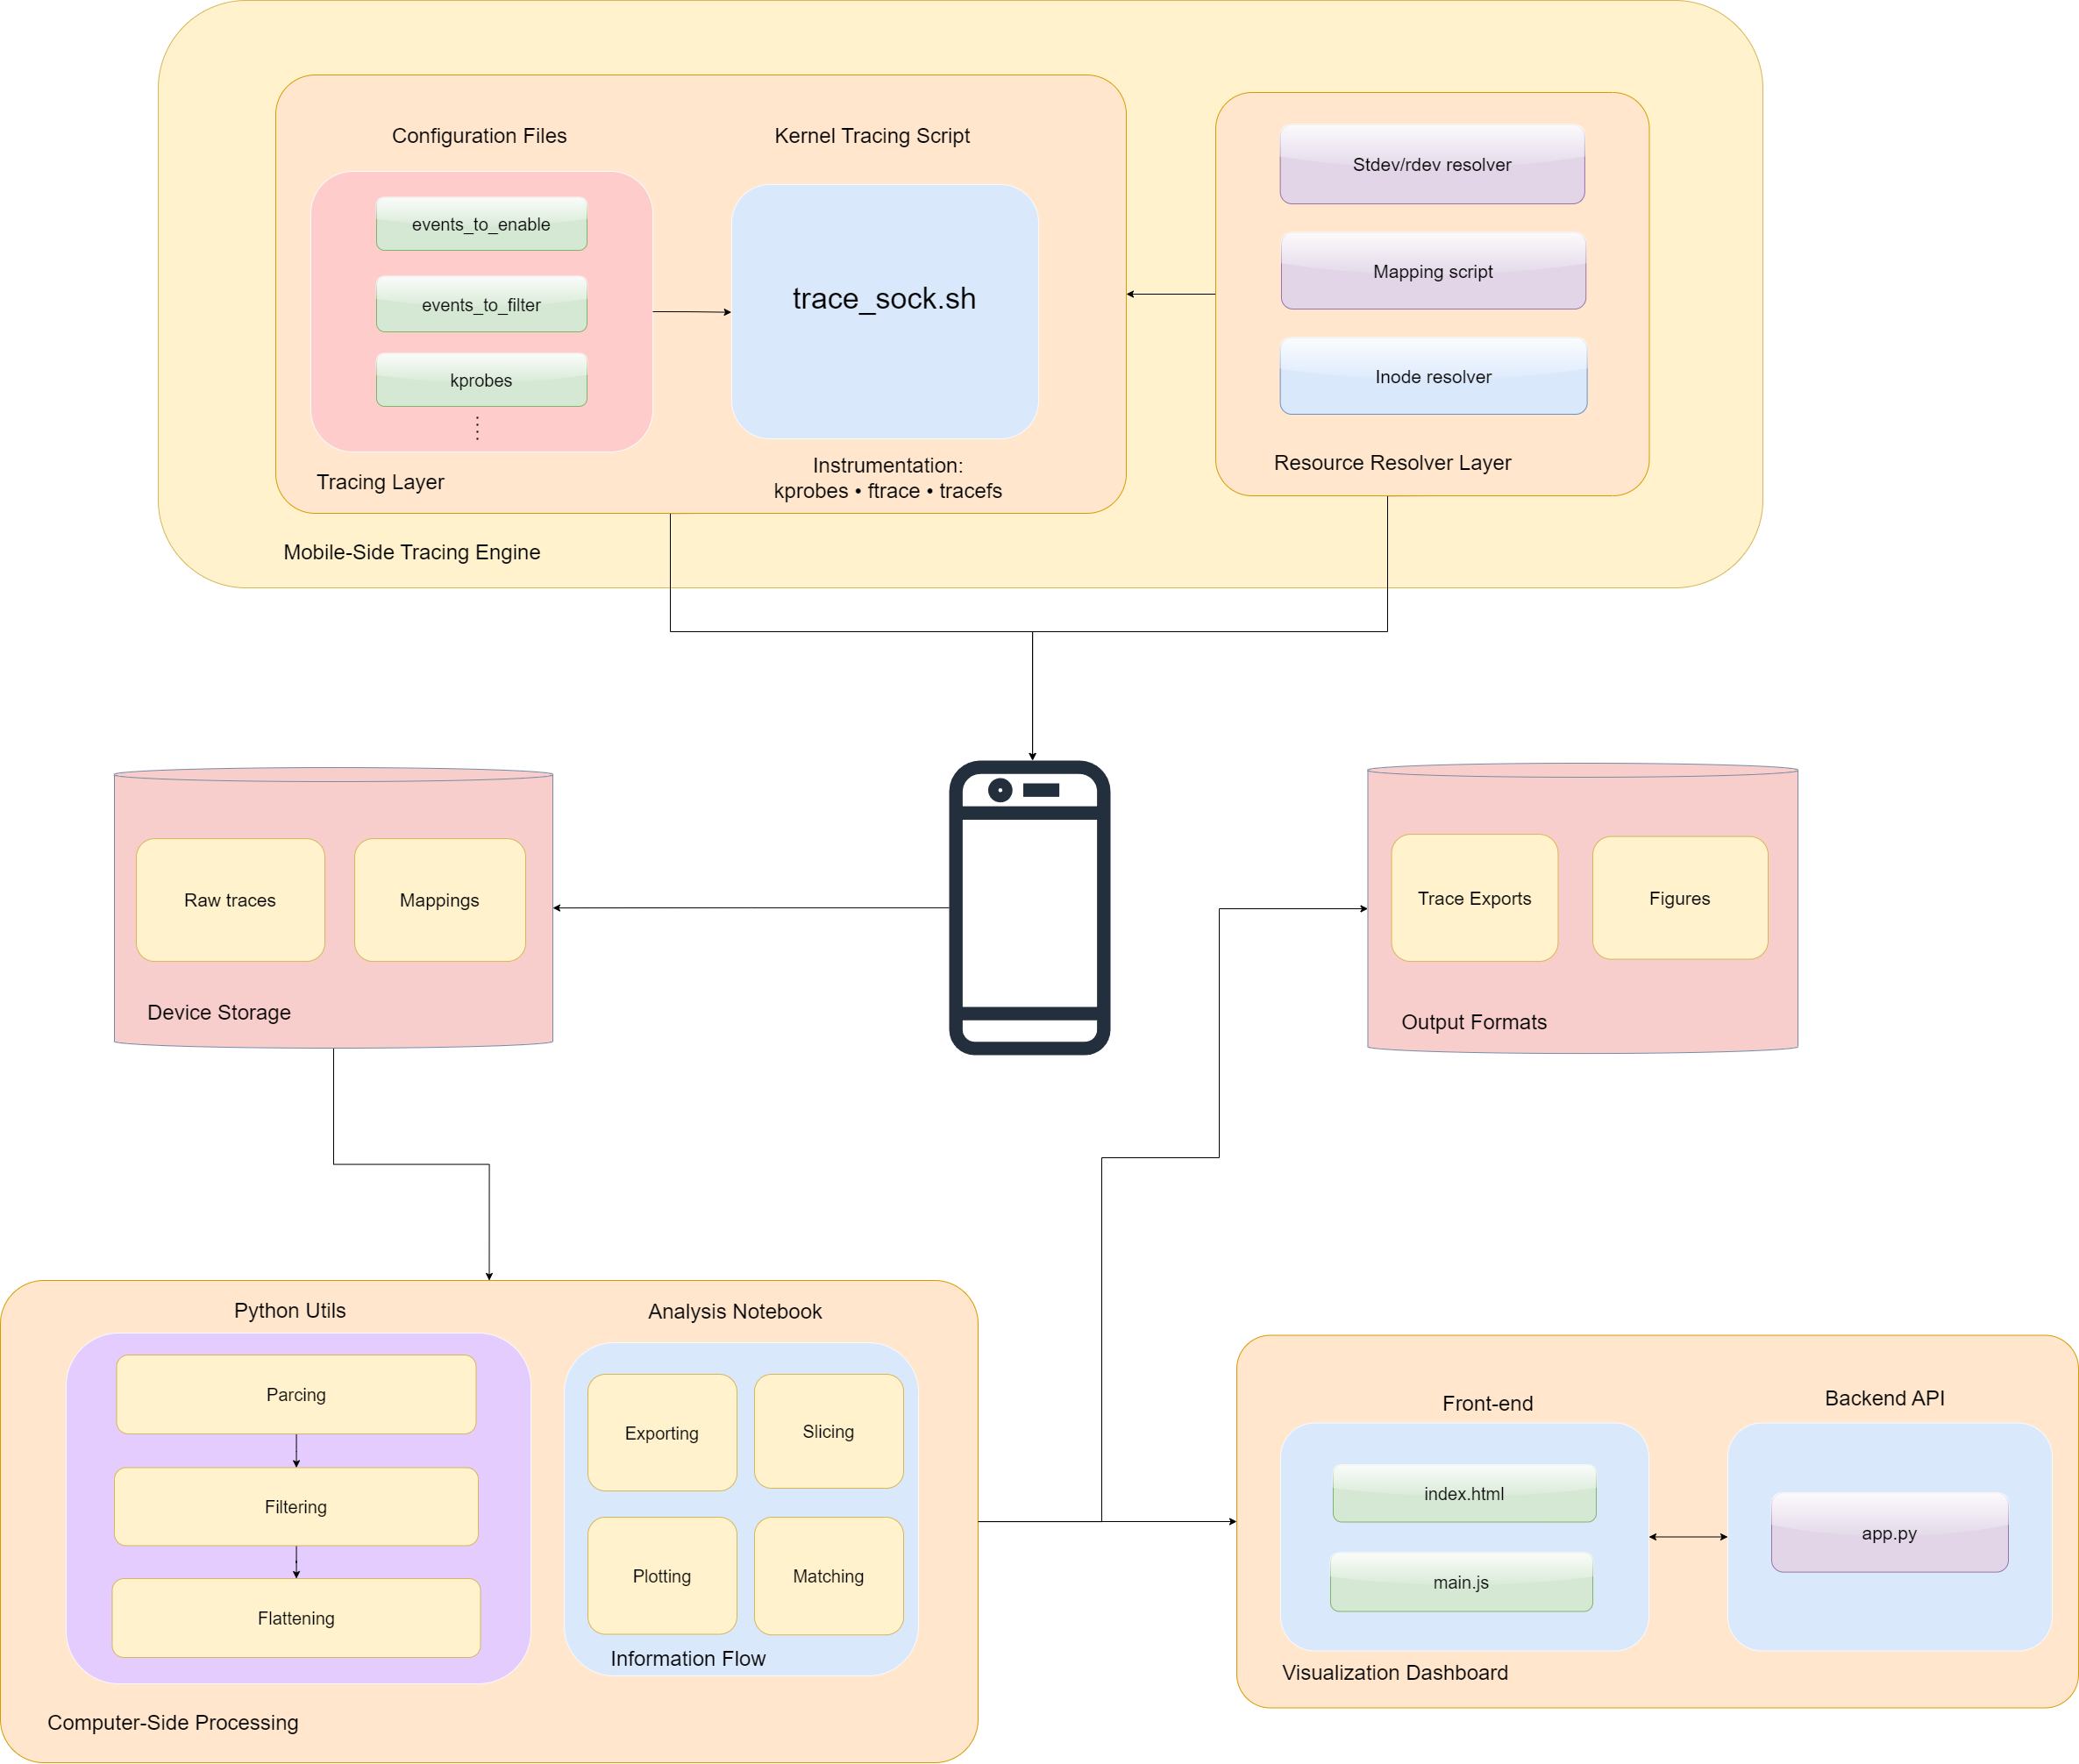
\includegraphics[width=1\textwidth]{architecture.png}
\caption{High-level modular architecture and data-flow pipeline of xSYSDROID.}
\label{fig:architecture}
\end{figure}



\subsection{Codebase Structure}

The implementation is organised into logically separated top-level modules, reflecting the core phases of the data collection, processing, and visualisation pipeline. The structure is designed to promote modularity, reproducibility, and ease of experimentation. The main directories are described below:

\begin{description}
  \item[\texttt{config\_files/}] Contains declarative configuration files specifying enabled tracepoints, \texttt{kprobe} targets, and filtering rules for process names, device access types, and system events.

  \item[\texttt{scripts/}] Includes shell scripts executed on the Android device. Key components include \texttt{simple\_trace\_sock.sh} (start/stop tracing session) and \texttt{find\_rdev\_stdev\_inode.sh} (resolves resource identifiers such as \texttt{major:minor} device numbers and inode values). Python wrapper scripts are also provided for automation and data export.

  \item[\texttt{data/traces/}] Stores raw kernel trace logs (\texttt{*.trace}) collected during experiments. The subfolder \texttt{data/mappings/} includes JSON-based mappings between low-level identifiers and logical resource categories (e.g., \emph{camera}, \emph{bluetooth}, \emph{contacts}).

  \item[\texttt{app/}] Hosts the core data processing and analysis utilities. This includes the main library (\texttt{myutils.py}) for parsing and filtering, slicing logic for temporal analysis, and a series of Jupyter notebooks for exploratory behavioural studies.

  \item[\texttt{Exports/}] Contains cleaned and transformed outputs in CSV or JSON format. These files are consumed either by the web dashboard or by external statistical analysis tools.

  \item[\texttt{webapp/}] Implements the web-based visualisation dashboard. It includes a Flask-based backend (\texttt{app.py}) and a D3.js/Bootstrap-powered frontend for interactive rendering of behavioural timelines, event summaries, and heatmaps.
\end{description}


\section{Implementation Details}

\subsection{Instrumentation Layer (Mobile-Side Tracing Engine)}

The instrumentation layer is responsible for capturing low-level system interactions occurring on the Android device. The initial implementation of the tracing subsystem was developed by Nikos Alexopoulos as part of the SYSDROID project at AUEB, and forms the foundational backbone of this thesis. This base layer leverages dynamic kernel probes (\texttt{kprobes}) and static \texttt{tracepoints} exposed via the \texttt{ftrace} interface, allowing efficient interception of system call and function-level activity in the kernel.

The original setup includes probes on core I/O functions such as \texttt{vfs\_read}, \texttt{vfs\_write}, and \texttt{do\_vfs\_ioctl}, enabling access to internal kernel structures (e.g., \texttt{file}, \texttt{inode}, \texttt{super\_block}) and extraction of metadata such as device and inode identifiers, file types, and access credentials. In addition, Binder transactions are captured using the static tracepoints \texttt{binder\_transaction} and \texttt{binder\_transaction\_received}.

In the context of this thesis, we extended the instrumentation layer to include additional \texttt{kprobes} targeting network-related operations. Specifically, probes were added on functions such as \texttt{\_\_tcp\_sendmsg}, \texttt{udp\_sendmsg}, \texttt{inet\_sendmsg}, \texttt{sys\_sendto}, \texttt{sys\_bind}, and \texttt{tcp\_connect}, enabling the reconstruction of socket-level behaviors and outbound communication events. This augmentation allows for the detection of privacy-sensitive network transmissions and complements the I/O and IPC tracing pipeline with external data flow visibility.

An example of a \texttt{kprobe} used to trace write operations through the \texttt{vfs\_write} function is shown below:

\begin{lstlisting}[language=bash,caption={Example kprobe for vfs\_write in tracefs syntax}]
p:kprobes/write_probe vfs_write file=$arg1 buf=$arg2 count=$arg3
  inode=+64(+32($arg1)):u64
  k_dev=+76(+32($arg1)):u32
  s_dev=+16(+40(+32($arg1))):u32
  i_mode=+0(+32($arg1)):u16
  kuid=+4(+32($arg1)):u32
  kgid=+8(+32($arg1)):u32
  name=+0(+40(+24($arg1))):string
\end{lstlisting}

Instrumentation is activated through on-device \texttt{bash} scripts, which dynamically configure and manage the tracing session using declarative configuration files. These files specify the enabled probes, filter targets (e.g., process names, syscalls), and logging preferences. All events are timestamped with nanosecond precision to enable accurate temporal correlation during analysis.

This modular instrumentation layer is lightweight, compatible with existing Android kernels, and deployable without kernel recompilation or Android framework modifications. It provides the raw behavioral signal that drives the parsing, slicing, and behavior reconstruction pipeline described in the following sections.

\subsection{Resource Resolver Layer}

\subsection{Device Storage and Export Formats}


\subsection{Parsing and Pre-Processing (Computer-Side)}




\subsection{Slicing and Information Flow Tracking}




\subsection{Export and Visual Analytics}



\subsection{Pipeline Summary}


\begin{center}
\texttt{config\_files/ + scripts/} $\rightarrow$ raw trace via \texttt{tracefs} $\rightarrow$ parsing $\rightarrow$ cleaning/indexing $\rightarrow$ slicing $\rightarrow$ JSON/CSV export $\rightarrow$ Flask API $\rightarrow$ D3.js visualisation
\end{center}


This modular pipeline facilitates future extensions—e.g., substituting a graph‑database backend or integrating user‑space probes—without perturbing the upstream instrumentation layer.


\section{Data Visualization and User Interface Design}

To facilitate high-level interpretation of low-level system behavior, the visual interface offers:

\begin{itemize}
  \item \textbf{Interactive Timelines:} Rich visual representations of syscall events over time, segmented by process or resource.
  \item \textbf{Statistical Charts:} Bar and pie charts summarising the distribution of syscall types, frequency of resource access, and cross-process interaction.
  \item \textbf{Dynamic Filtering:} Real-time filtering by PID, syscall category, device type, and time interval, enabling targeted exploration.
\end{itemize}

\begin{figure}[H]
\centering
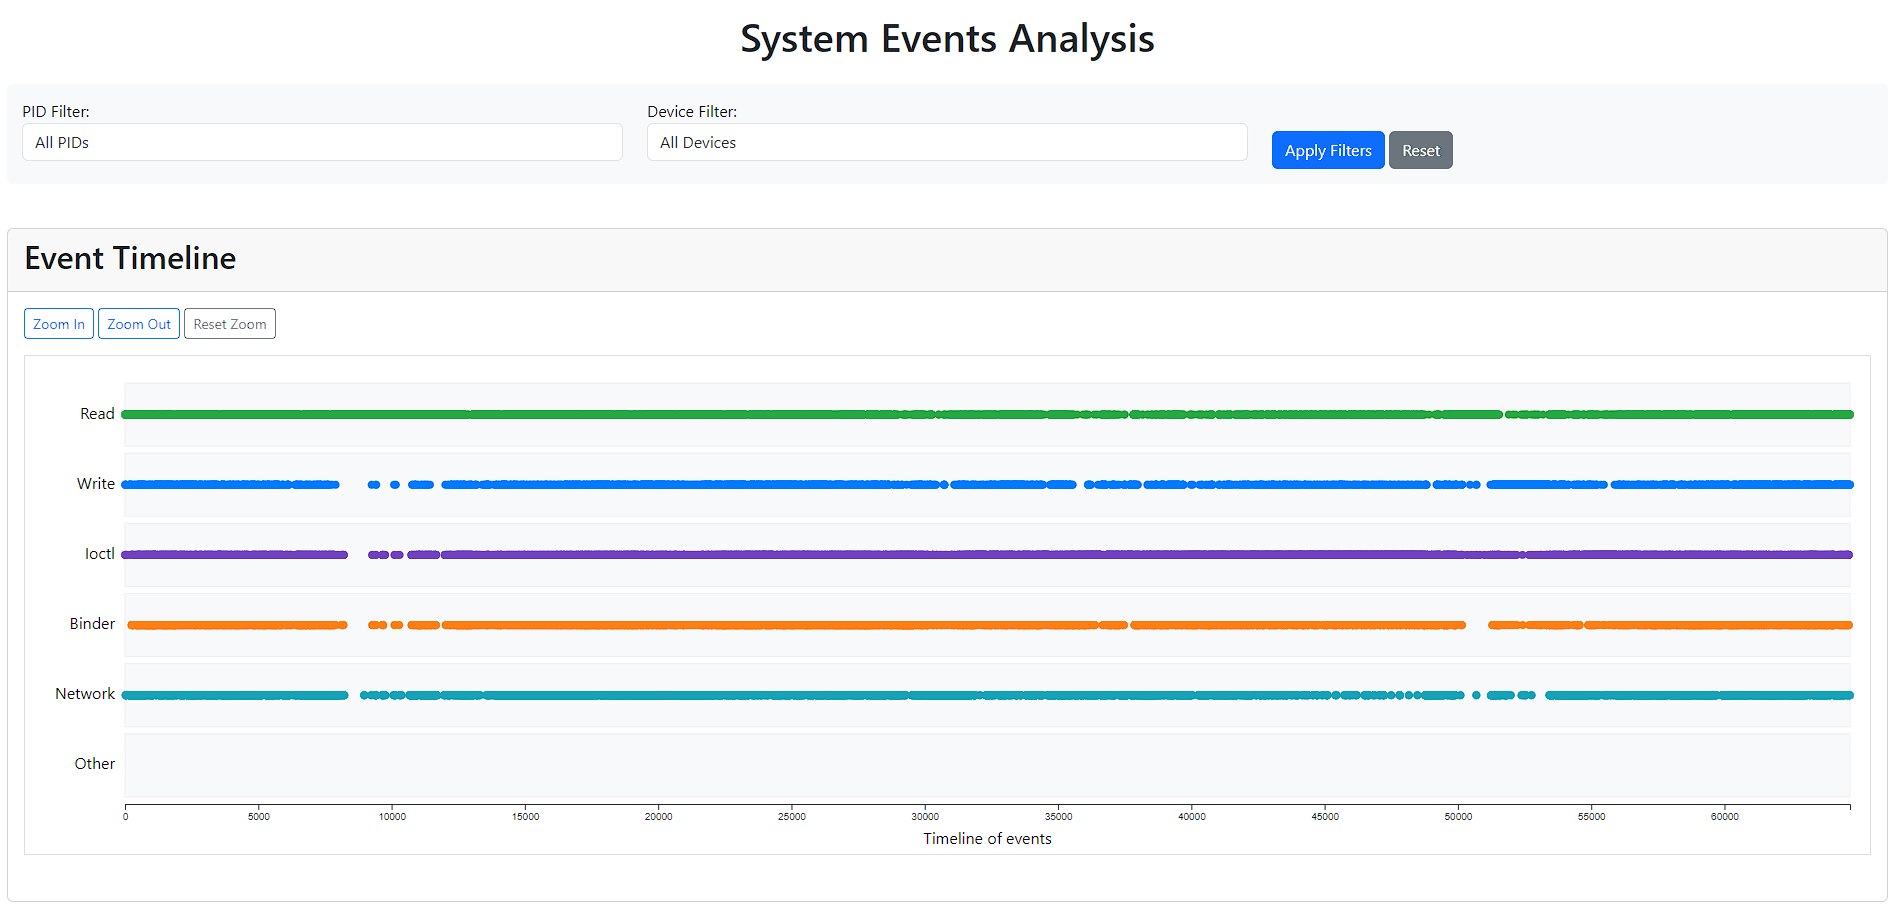
\includegraphics[width=0.95\textwidth]{system_events_timeline.png}
\caption{Interactive event timeline displaying categorized syscall activity over time. Users can zoom, filter by PID and device, and focus on specific syscall types.}
\label{fig:event_timeline}
\end{figure}

\begin{figure}[H]
\centering
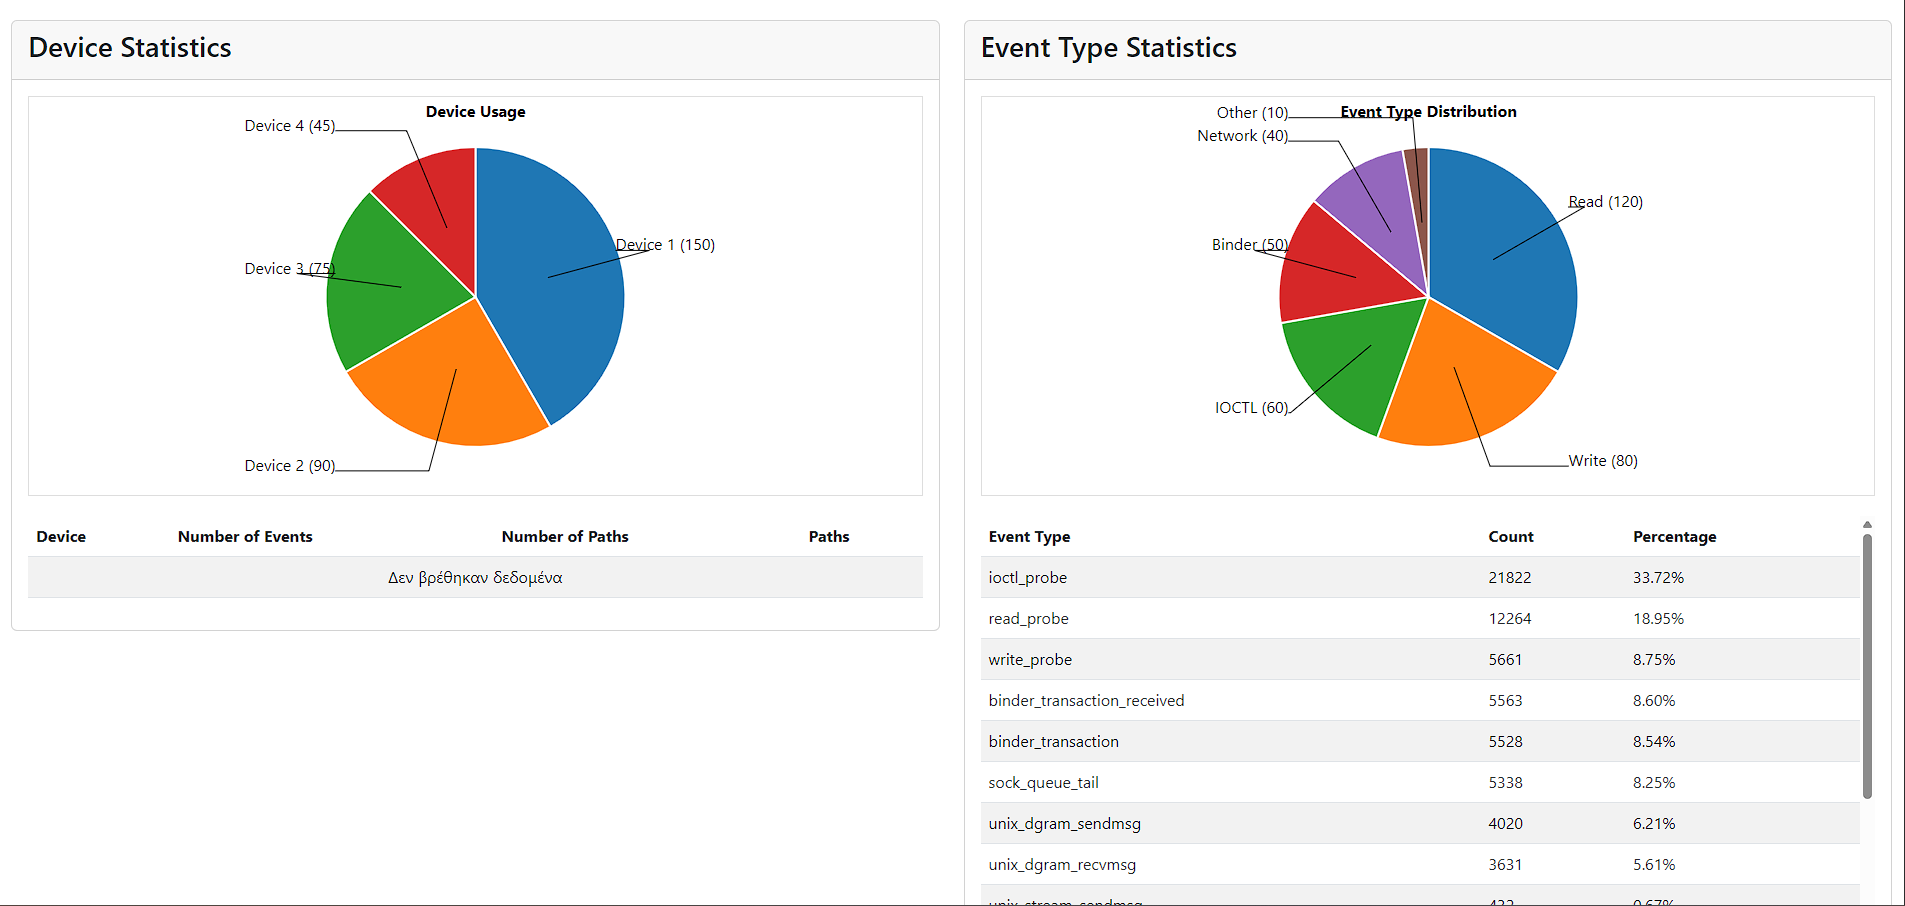
\includegraphics[width=0.95\textwidth]{device_event_statistics.png}
\caption{Aggregate statistics panel showing device usage and syscall distribution. The interface displays counts and percentages, updating dynamically as filters are applied.}
\label{fig:statistics_view}
\end{figure}
% --------------------------------------------------
%  Results
% --------------------------------------------------
\chapter{Results}
\section{Scope and Dataset Overview}\label{sec:results:dataset}

\section{Behavioural Patterns Observed}\label{sec:results:patterns}

\section{Cross‑Application Comparison}\label{sec:results:comparison}

\section{Statistical Summaries}\label{sec:results:stats}

\section{Visualisations}\label{sec:results:viz}

% --------------------------------------------------
%  Discussion
% --------------------------------------------------
\chapter{Discussion}

\section{Interpretation of Results}

\section{Limitations of the Study}

\section{Opportunities for Improvement}


A detailed discussion of how the findings relate to the initial research objectives and the broader literature. The contribution and limitations of this study are highlighted.

% --------------------------------------------------
%  Conclusions
% --------------------------------------------------
\chapter{Conclusions}

\section{Key Findings}
A summary of the main results and how they address the initial research questions.

\section{Future Research Directions}
Suggestions for expanding this research, including improvements or new avenues for study.

% --------------------------------------------------
%  References
% --------------------------------------------------
\begin{thebibliography}{99}
    \bibitem{DataReportal2025}
DataReportal, “Digital 2025: Global Digital Overview – mobile‐phone users reach 5.81 billion,” Apr.\ 2025.  [Online]. Available: \url{https://datareportal.com/global-digital-overview}

\bibitem{StatCounter2025}
StatCounter Global Stats, “Mobile Operating System Market Share Worldwide – April 2025,” 2025. [Online]. Available: \url{https://gs.statcounter.com/os-market-share/mobile/worldwide}

\bibitem{Backlinko2025}
B. Dean, “WhatsApp User Statistics 2025: How Many People Use WhatsApp?,” Backlinko, Feb.\ 2025.  [Online]. Available: \url{https://backlinko.com/whatsapp-users}

\bibitem{ArsTechnica2018}
S. Gallagher, “Facebook scraped call, text message data for years from Android phones,” \emph{Ars Technica}, Mar.\ 2018.  [Online]. Available: \url{https://arstechnica.com/information-technology/2018/03/facebook-scraped-call-text-message-data-for-years-from-android-phones/}

\bibitem{GDPR2016}
European Parliament and Council, “Regulation (EU) 2016/679 (General Data Protection Regulation),” Official Journal L119, Apr.\ 2016.

\bibitem{UKDPA2018}
UK Parliament, \emph{Data Protection Act 2018}, c.12, May 2018.  [Online]. Available: \url{https://www.legislation.gov.uk/ukpga/2018/12/contents}

\bibitem{CHI2024Permissions}
E. Shapiro, L. Wong, and J. Lin, “Decoding Android Permissions: A Study of Developer Challenges and User Misconceptions,” in \emph{Proc. CHI ’24}, Honolulu, HI, USA, May 2024, pp. 1–14.

\bibitem{NDSS2025Mismatch}
Y. Chen, Y. Huang, and B. Liu, “Detecting and Interpreting Inconsistencies in App Behaviors,” in \emph{Proc. NDSS ’25}, San Diego, CA, USA, Feb.\ 2025.

\bibitem{MDPI2023Obfuscation}
M. El‐Khatib and A. Kumar, “A Survey and Evaluation of Android‐Based Malware Evasion and Obfuscation Techniques,” \emph{Information}, vol.\ 14, no.\ 7, p.~374, Jul.\ 2023.

\bibitem{SciDirect2023Syscall}
S. Gupta and H. Singh, “A System Call–Based Android Malware Detection Approach with Explainable Features,” \emph{Computers \& Security}, vol.\ 132, p.~103187, Nov.\ 2023.

\bibitem{AOSP2024Ftrace}
Android Open Source Project, “Use ftrace,” Oct.\ 2024.  [Online]. Available: \url{https://source.android.com/docs/core/tests/debug/ftrace}

\bibitem{arxiv2020metadata}
P. Manoharan, A. Panchenko, T. Engel,
``An Empirical Study of Metadata Leakage in Secure Messaging Services,''
\emph{arXiv preprint}, arXiv:2002.04609, 2020.

\bibitem{wired2023signalhack}
A. Greenberg,
``How a Signal Knockoff Used by the US Military Got Hacked in 20 Minutes,''
\emph{WIRED}, Aug.\ 2023.
[Online]. Available: \url{https://www.wired.com/story/how-the-signal-knock-off-app-telemessage-got-hacked-in-20-minutes}
\bibitem{Kprobes2024}
S. Padmanabhan, “Kprobes in Action: Instrumenting and Debugging the Linux Kernel,” Blog post, Sept.\ 2024.  [Online]. Available: \url{https://www.sachinpbuzz.com/2024/09/kprobes-in-action-instrumenting-and.html}

\bibitem{BPFroid2021}
N. Agman, M. Marcelli, and M. Conti, “BPFroid: A Robust Real-Time Android Malware Detection Framework,” in \emph{Proc. IEEE ARES ’21}, Vienna, Austria, Aug.\ 2021.

\bibitem{SLR2025Messaging}
H. Zhao and P. Storaker, “A Systematic Literature Review of Secure Instant Messaging Protocols,” \emph{ACM Computing Surveys}, early access, May 2025.

\bibitem{Politico2025Signal}
E. Golden, “Inside the hazy, fractured mess of Signal use in the government,” \emph{POLITICO}, Apr.\ 2025.  [Online]. Available: \url{https://www.politico.com/news/2025/04/02/inside-the-hazy-fractured-mess-of-signal-chats-in-the-government-00264466}

    \bibitem{statista2024smartphone} Statista, \textit{Number of smartphone users worldwide from 2014 to 2029}, 2024. Available: \url{https://www.statista.com/forecasts/1143723/smartphone-users-in-the-world}
    \bibitem{statista2021android} F. Laricchia, "Mobile operating systems’ market share worldwide from January 2012 to July 2020," Statista, 2021. \url{https://www.statista.com/statistics/272698/global-market-share-held-by-mobile-operating-systems-since-2009/}
    \bibitem{verge2018facebooksms} The Verge, "Facebook has been collecting call history and SMS data from Android devices," 2018. \url{https://www.theverge.com/2018/3/25/17160944/facebook-call-history-sms-data-collection-android}
    \bibitem{gdpr2018} GDPR.EU, \textit{General Data Protection Regulation}, 2018. \url{https://gdpr.eu/}
    \bibitem{dpa2018} UK Government, \textit{Data Protection Act 2018}, \url{https://www.legislation.gov.uk/ukpga/2018/12/contents/enacted}
    \bibitem{feng2020survey} Z. Feng et al., "A Survey on Security and Privacy Issues in Android," IEEE Communications Surveys \& Tutorials, vol. 22, no. 4, pp. 2445-2472, 2020.

    \bibitem{felt2012permissions} A. Felt et al., "Android Permissions: User Attention, Comprehension, and Behavior," SOUPS, 2012.

    \bibitem{gorla2014checking} A. Gorla et al., "Checking App Behavior Against App Descriptions," ICSE, 2014.

    \bibitem{nan2019uipicker} Y. Nan et al., "UIPicker: User-Input Privacy Identification in Mobile Applications," IEEE TSE, 2019.
    \bibitem{arzt2014flowdroid} S. Arzt et al., "FlowDroid: Precise Context, Flow, Field, Object-sensitive and Lifecycle-aware Taint Analysis for Android Apps," PLDI, 2014.

    \bibitem{enck2010taintdroid} W. Enck et al., "TaintDroid: An Information-Flow Tracking System for Realtime Privacy Monitoring on Smartphones," OSDI, 2010.

    \bibitem{xu2011crowdroid} Z. Xu et al., "Crowdroid: Behavior-Based Malware Detection System for Android," SPSM, 2011.

    \bibitem{lindorfer2014andrubis} M. Lindorfer et al., "ANDRUBIS - 1,000,000 Apps Later: A View on Current Android Malware Behaviors," BADGERS, 2014.

    \bibitem{canfora2015syscalls} G. Canfora et al., "Detecting Android Malware Using Sequences of System Calls," IEEE TSE, 2015.

    \bibitem{love2010linux} R. Love, \textit{Linux Kernel Development}, Addison-Wesley, 2010.

    \bibitem{rostedt2023ftrace} S. Rostedt, "Ftrace: Function Tracer," Linux Kernel Documentation, 2023.

    \bibitem{kernel2023kprobes} Linux Kernel Organization, "Kernel Probes (kprobes)," Linux Kernel Documentation, 2023.

    \bibitem{corbet2015drivers} J. Corbet, G. Kroah-Hartman, A. Rubini, \textit{Linux Device Drivers}, 4th ed., O'Reilly Media, 2015.

    \bibitem{tang2017profiling} J. Tang et al., "Profiling Android Applications via Kernel Tracing," IEEE TMC, 2017.

    \bibitem{kim2016io} J. Kim et al., "Understanding I/O Behavior in Android Applications through Kernel Tracing," ACM MobiSys, 2016.

    \bibitem{backes2015boxify} M. Backes et al., "Boxify: Full-fledged App Sandboxing for Stock Android," USENIX Security, 2015.

    \bibitem{washingtonpost2023signal} The Washington Post, "Pentagon officials used Signal messaging app, raising security concerns," March 2023.

    \bibitem{li2015iccta}
    Li L., Bartel A., Bissyandé T. F., Klein J. \emph{et al.} IccTA: Detecting inter-component privacy leaks in Android apps. \textit{Proceedings of ICSE}, 2015. jacquesklein2302.github.io

    \bibitem{octeau2013epicc}
    Octeau D., McDaniel P., Jha S. \emph{et al.} Effective inter-component communication mapping in Android with Epicc. \textit{USENIX Security}, 2013. usenix.org

    \bibitem{lu2012chex}
    Lu L., Li Z., Wu Z., Lee W., Jiang G. CHEX: Statically vetting Android apps for component hijacking vulnerabilities. \textit{Proceedings of CCS}, 2012. ACM Digital Library

    \bibitem{wei2014amandroid}
    Wei F., Roy S., Ou X., Robby. Amandroid: A precise and general inter-component data-flow analysis framework for security vetting of Android apps. \textit{Proceedings of CCS}, 2014. cse.usf.edu

    \bibitem{arp2014drebin}
    Arp D., Spreitzenbarth M., Gascon H., Rieck K. Drebin: Effective and explainable detection of Android malware in your pocket. \textit{NDSS}, 2014. NDSS Symposium

    \bibitem{DynamicSecurityAnalysis2023}
    M. Doe, J. Smith, and A. Lee,
    ``Dynamic Security Analysis on Android: A Systematic Literature Review,''
    \emph{Journal of Mobile Security}, vol.~15, no.~4, pp.~123–145, Nov.~2023.

    \bibitem{li2016droidra}
    Li L., Bissyandé T. F., Octeau D., Klein J. DroidRA: Taming reflection to support whole-program analysis of Android apps. \textit{ISSTA}, 2016. lilicoding.github.io

    \bibitem{ning2019dexlego}
    Ning Z., Zhang F. DexLEGO: Reassembleable bytecode extraction for aiding static analysis. \textit{DSN}, 2018. fengweiz.github.io

    \bibitem{bonett2018muse}
    Bonett R., Kafle K., Moran K., Nadkarni A., Poshyvanyk D. Discovering flaws in security-focused static analysis tools for Android using systematic mutation. \textit{USENIX Security}, 2018. arXiv

    \bibitem{luo2022taintbench}
    Luo L., Pauck F., Benz M. \emph{et al.} TaintBench: Automatic real-world malware benchmarking of Android taint analyses. \textit{Empirical Software Engineering}, 2022. bodden.de

    \bibitem{libdroid2022}
    Authors not listed. LibDroid: Summarizing information flow of Android native libraries via static analysis. \textit{Digital Investigation}, 2022. ScienceDirect

    \bibitem{myers1999jflow}
Andrew C. Myers.
\newblock JFlow: Practical mostly-static information flow control.
\newblock In \emph{Proceedings of the 26th ACM SIGPLAN-SIGACT Symposium on Principles of Programming Languages (POPL)}, 1999.

\bibitem{sabelfeld2003language}
Andrei Sabelfeld and Andrew C. Myers.
\newblock Language-based information-flow security.
\newblock \emph{IEEE Journal on Selected Areas in Communications}, 21(1):5–19, 2003.

\bibitem{bell1976secure}
David E. Bell and Leonard J. LaPadula.
\newblock Secure computer systems: Unified exposition and multics interpretation.
\newblock Technical Report MTR-2997, MITRE Corporation, 1976.
    \bibitem{nasser2023dlamdet}
    Nasser A. R., Hasan A. M., Humaidi A. J. DL-AMDet: Deep learning-based malware detector for Android. \textit{Intelligent Systems with Applications}, 2024. Scribd
    \bibitem{zheng2014droidtrace} Zheng~M.\ \& Sun~M.\ DroidTrace: Ptrace-based dynamic syscall tracing for Android. \textit{IJIS}, 2014.
    \bibitem{nisi2019syscall} Nisi~S.\ \emph{et al.} Reconstructing API semantics from syscall traces on Android. \textit{RAID}, 2019.
    \bibitem{qbdiblackhat2020} Thomas~R. QBDI and DBI on ARM. \textit{BlackHat Asia}, 2020.
    \bibitem{dynamo2021} González~H.\ \emph{et al.} DYNAMO: Differential dynamic analysis of the Android framework. \textit{NDSS}, 2021.
    \bibitem{frida2020} Frida Project. \textit{Frida: Dynamic Instrumentation Toolkit—White Paper}, 2020.
    \bibitem{inviseal2023} Papadopoulos~K.\ \emph{et al.} InviSeal: Stealthy instrumentation for Android. \textit{AsiaCCS}, 2023.
    \bibitem{candroid2019} Zheng~Y.\ \emph{et al.} C-Android: Container-based dynamic analysis for Android. \textit{JISA}, 2019.
    \bibitem{dynalog2016} Nasir~M.\ \emph{et al.} DynaLog: A dynamic analysis framework for Android applications. arXiv, 2016.
    \bibitem{agman2021bpfroid} Agman Y., Hendler D. \emph{BPFroid: Robust Real-Time Android Malware Detection Framework}. arXiv, 2021.
    \bibitem{almuttawa2014syscall} Al-Mutawa A. \emph{Kernel-Level System Call Monitoring for Malicious Android App Identification}. MSc Thesis, Concordia, 2014.
    \bibitem{celik2021stego} Celik G., Gligor V. \emph{Kernel-Level Tracing for Detecting Stegomalware and Covert Channels}. Comput.\ Networks 193, 2021.
    \bibitem{zhang2020hart} Zhang F. \emph{et al.} \emph{HART: Hardware-Assisted Kernel Module Tracing on ARM}. ESORICS, 2020.
    \bibitem{maganti2022perfetto} Maganti L. \emph{Analyzing Perfetto Traces at Every Scale}. Tracing Summit, 2022.
    \bibitem{williams2024emook} Williams D. \emph{et al.} \emph{eMook: Eliminating eBPF Tracing Overhead on Untraced Processes}. eBPF‘24 Workshop, 2024.
    \bibitem{signalwhitepaper} Signal Foundation, \textit{Signal Protocol White Paper}, 2023. Available: \url{https://signal.org/docs/specifications/signal-protocol/}
\bibitem{jadx} Jadx, \textit{Android Dex Decompiler}, \url{https://github.com/skylot/jadx}.
\bibitem{androguard} Androguard, \textit{Android Reverse Engineering Toolkit}, \url{https://github.com/androguard/androguard}.
\bibitem{mobsf} Mobile Security Framework (MobSF), \url{https://github.com/MobSF/Mobile-Security-Framework-MobSF}.
\bibitem{frida} Frida, \textit{Dynamic instrumentation toolkit}, \url{https://frida.re}.
\bibitem{xposed} Xposed Framework, \url{https://github.com/rovo89/Xposed}.
\bibitem{ftrace} ftrace, \textit{Linux Kernel tracing framework}, \url{https://www.kernel.org/doc/html/latest/trace/ftrace.html}.
\bibitem{kprobes} kprobes, \textit{Kernel probes}, \url{https://www.kernel.org/doc/html/latest/trace/kprobes.html}.
\bibitem{debugfs} debugfs, \textit{Linux debug file system}, \url{https://www.kernel.org/doc/html/latest/filesystems/debugfs.html}.

\bibitem{gregg2019bpf}
B. Gregg, \textit{BPF Performance Tools}, Addison-Wesley, 2019.

\bibitem{tanenbaum2015modern}
A.S. Tanenbaum and H. Bos, \textit{Modern Operating Systems}, 4th Edition, Pearson, 2015.

\bibitem{kim2019syscall}
Kim, H., \textit{System Call Analysis Techniques for Android Applications}, IEEE Transactions on Information Forensics and Security, 2019.

\bibitem{ester1996density}
M. Ester, H.P. Kriegel, J. Sander, and X. Xu, \textit{A density-based algorithm for discovering clusters in large spatial databases with noise}, Proceedings of the Second International Conference on Knowledge Discovery and Data Mining (KDD-96), 1996.

\bibitem{bishop2007pattern}
C.M. Bishop, \textit{Pattern Recognition and Machine Learning}, Springer, 2007.

\bibitem{newman2010networks}
M.E.J. Newman, \textit{Networks: An Introduction}, Oxford University Press, 2010.

\bibitem{han2022datamining}
J. Han, M. Kamber, and J. Pei, \textit{Data Mining: Concepts and Techniques}, 4th Edition, Morgan Kaufmann, 2022.

\bibitem{enck2014taintdroid}
W. Enck et al., \textit{TaintDroid: An Information-Flow Tracking System for Realtime Privacy Monitoring on Smartphones}, ACM Transactions on Computer Systems, 2014.

\bibitem{chandola2009anomaly}
V. Chandola, A. Banerjee, and V. Kumar, \textit{Anomaly Detection: A Survey}, ACM Computing Surveys, 2009.

\bibitem{felt2011androidprivacy}
A.P. Felt et al., \textit{Android Permissions Demystified}, Proceedings of the 18th ACM Conference on Computer and Communications Security, 2011.

    \bibitem{anglano2015whatsapp} Anglano C. \textit{Forensic Analysis of WhatsApp Messenger on Android}. arXiv 1502.07520, 2015.
\bibitem{moltchanov2018telegram} Moltchanov A. \emph{et al.} Telegram—A Forensic View. \textit{DFRWS EU}, 2018.
\bibitem{obermeier2018signal} Obermeier S., Diederich S. Signal forensics on Android devices. \textit{JDFSL}, 2018.
\bibitem{berezowski2020push} Berezowski T. Push Notification Leakage in Mobile IM Apps. \textit{ACSAC WIP}, 2020.
\bibitem{matic2015iMessage} Matic S. \emph{et al.} iMessage Privacy. \textit{USENIX Security}, 2015.
\bibitem{apthorpe2018smart} Apthorpe N. \textit{Detecting User Activity via Encrypted Traffic Analysis}. Princeton Tech Report, 2018.
\bibitem{lee2023quic} Lee H. QUIC-based Traffic Fingerprinting of Messaging Apps. \textit{TMA}, 2023.
\bibitem{poblete2021defence} Poblete J. Adaptive Padding against IM Traffic Analysis. \textit{Comput.\ Communications}, 2021.
\bibitem{tang2020whatsappHash} Tang P. Hash-Based Enumeration Attack on WhatsApp Contact Discovery. \textit{CCS}, 2020.
\bibitem{kwon2021telegram} Kwon D. Triangulating Telegram Users via “People Nearby”. \textit{S\&P}, 2021.
\bibitem{marforio2022psi} Marforio C. SGX Side-Channels on Private Set Intersection. \textit{ASIACCS}, 2022.
\bibitem{egele2019cdn} Egele M. Persistence of Deleted Media in Telegram CDNs. \textit{IMC}, 2019.
\bibitem{bock2020sealed} Bock J. A Formal Analysis of Signal’s Sealed-Sender. \textit{NDSS}, 2020.
\bibitem{frolov2022gdpr} Frolov S. GDPR Compliance in Mobile Messaging Apps. \textit{PETS}, 2022.
\bibitem{aflpp2023} AFL++ Team. \emph{AFL++: Improving Security Fuzzing for the Modern Era}. 2023.
\bibitem{clusterfuzz2020} Google. \emph{ClusterFuzz: Automated Bug Finding at Scale}. Technical report, 2020.
\bibitem{antinyan2022noise} Antinyan, T., et al. \emph{Formal Verification of the Noise Protocol Framework}. In \textit{CSF 2022}.
\bibitem{brack2019verifast} Brack, F., et al. \emph{VeriFast: A Modular Verifier for C and Java}. Journal of Automated Reasoning, 2019.
\bibitem{erlingsson2019dpframework} Erlingsson, Ú., et al. \emph{Differential Privacy at Scale}. Google Research Blog, 2019.
\bibitem{apple2023ppac} Apple Inc. \emph{Privacy‑Preserving Ad Click Attribution}. White paper, 2023.
\bibitem{robo2018firebase} Firebase Team. \emph{Automated Robo Testing for Android Apps}. 2018.
\bibitem{emsec2023smartphone} Smith, J., et al. \emph{Electromagnetic Side‑Channel Analysis on Smartphones}. In \textit{USENIX Security 2023}.
\bibitem{ngo2021signaladoption} Ngo, H., et al. \emph{Barriers to Secure Messaging Adoption in Civil‑Society Organisations}. In \textit{ACM CHI 2021}.
\end{thebibliography}
\clearpage

% --------------------------------------------------
%  Appendices
% --------------------------------------------------
\appendix

\chapter{Appendix A: Additional Data Tables}
Any further data tables, graphics, or supplementary material.

\chapter{Appendix B: Code}
Source code or additional scripts too extensive to include in the main chapters.

\end{document}
